\documentclass[11pt]{article}
\usepackage[margin=1in]{geometry}
\usepackage{pdfpages}
\usepackage{hyperref}
\hypersetup{colorlinks=true,linkcolor=blue,urlcolor=blue}
\pagestyle{empty}

\begin{document}

% ================================================================
% COVER LETTER
% ================================================================
\vspace*{2cm}

\begin{center}
{\LARGE HyperTensor Papers I--XIX}

\vspace{10pt}

William Ken Ohara Stewart

NagusameCS Independent Research

\texttt{nagusamecs@gmail.com}

\url{https://github.com/NagusameCS/HyperTensor}

\vspace{10pt}

May 2026
\end{center}

\vspace{18pt}

To whom it may concern,

\vspace{8pt}

Thank you for taking the time to look through this work. My name is William
Ken Ohara Stewart. I am eighteen years old and a high school student in the
United States. I am not a professional researcher, I do not have a lab or an
advisor, and I am certain there are mistakes in these pages that a trained eye
would catch immediately. I ask for your patience with those. Everything here
was done on a laptop with an RTX 4070, a rented cloud GPU when a bigger one was
needed, and a lot of late nights.

What follows is a set of ten papers that try to answer one question: can you
compress a language model using only the geometry of its own weights, with no
training data and no calibration, and still have it work? The answer, as of
Paper~X, is a qualified yes---but the qualification matters more than the yes
itself.

\vspace{10pt}

\section*{Summary of Papers}

\noindent Paper~I --- Geodesic Runtime Compression.
The core measurement. We compress only the attention weights (Q, K, V) of
Llama-3.1-8B by projecting them onto their own principal components, with no
calibration data. At one compression rank, the compressed model runs about six
percent faster than the uncompressed model on a laptop GPU. At a slightly larger
rank, throughput matches baseline and perplexity goes up by about thirteen
percent. The paper is honest about what is measured and what is not.

\vspace{4pt}

\noindent Paper~II --- Geodesic Projection Pipeline.
Extends the compression from three attention slots to all seven compressible
matrices in a transformer block, adds per-layer rank allocation, and describes
four adaptive mechanisms. Only the MCR mechanism has been tested, and it was a
null result at the tested rank. The remaining mechanisms are design
specifications, not measurements.

\vspace{4pt}

\noindent Paper~III --- Speculative Decoding with Compression.
Combines the compressed drafter from Paper~I with standard speculative decoding.
On SmolLM2-135M we measure a $1.53{\times}$ speedup at about thirty-nine percent
acceptance rate. One finding is negative: aggressive compression and speculative
decoding do not compose well.

\vspace{4pt}

\noindent Paper~IV --- Organic Training Theory.
The theoretical backbone. Proposes modeling transformer latent space as a
Riemannian manifold with the Fisher information metric where inference becomes
approximate geodesic flow. Twelve of seventeen testable claims now have measured
anchors across three model scales.

\vspace{4pt}

\noindent Paper~V --- GRC Light Distillation.
An optional distillation step recovering perplexity lost to compression.
On SmolLM2-135M, a small LoRA adapter recovers over one hundred percent of the
PPL gap at $k{=}512$. At aggressive compression recovery is partial.

\vspace{4pt}

\noindent Paper~VI --- Task-Level Impact.
Measures what happens to benchmark scores when you compress attention.
Knowledge recall holds up reasonably well down to $k{=}512$, but reasoning tasks
degrade sharply. An earlier MMLU measurement at $k{=}256$ was retracted.

\vspace{4pt}

\noindent Paper~VII --- FFN Cluster Compression.
Attempts structure-aware compression of the feed-forward network using column
clustering plus per-cluster SVD. Four-cluster compression reduces reconstruction
error by about twenty-three percent versus global SVD. Includes a correction
from an earlier overoptimistic prediction.

\vspace{4pt}

\noindent Paper~VIII --- GTC as RAG Alternative.
Explores whether the geodesic trajectory cache from Paper~IV can serve as a
retrieval mechanism. The computed speedup is large on paper but cross-model
generalization has not been measured.

\vspace{4pt}

\noindent Paper~IX --- The 106\% Anomaly as a General Phenomenon.
Argues that the super-baseline speedup from Paper~I is not a quirk. Derives the
condition under which compressed kernels run faster, predicts optimal ranks for
ten GPU types, and identifies six kernel classes beyond attention.

\vspace{4pt}

\noindent Paper~X --- Cross-Embedding Compatibility Index.
Tests whether you can splice parts of different models together by aligning their
embedding spaces. A working chimera called MINSKAT was built and published.
Within-model splicing fails at low compression ranks.

\vspace{14pt}

Thank you again for reading. If you find errors, they are mine. If you find
something useful, the credit belongs to the professors who have taught me, my
friends who told me which parts made no sense, and my parents who put up with
my waffling.

\vspace{8pt}

\begin{flushright}
William Ken Ohara Stewart

May 2026
\end{flushright}

\clearpage

% ================================================================
% CONTENTS
% ================================================================
\begin{center}
{\Large Contents}
\end{center}

\vspace{12pt}

\noindent Paper~I \hfill Geodesic Runtime Compression and the 106\% Baseline Anomaly

\noindent Paper~II \hfill Geodesic Projection Pipeline and MCR Allocation

\noindent Paper~III \hfill Composing Compression with Geodesic Speculative Decoding

\noindent Paper~IV \hfill Organic Training Theory and the Manifold Hypothesis

\noindent Paper~V \hfill GRC Light Distillation for Perplexity Recovery

\noindent Paper~VI \hfill Task-Level Impact of Geodesic Runtime Compression

\noindent Paper~VII \hfill Structure-Aware FFN Compression via Column Clustering

\noindent Paper~VIII \hfill Geodesic Trajectory Caching as an Alternative to RAG

\noindent Paper~IX \hfill The 106\% Anomaly as a General GPU Phenomenon

\noindent Paper~X \hfill Cross-Embedding Compatibility Index

\vspace{12pt}

\clearpage
\tableofcontents
\clearpage

\clearpage

% ================================================================
% PAPERS (included via pdfpages)
% ================================================================

\phantomsection\addcontentsline{toc}{section}{Paper I: Geodesic Runtime Compression}

\includepdf[pages=-,pagecommand={\thispagestyle{empty}}]{paper-I/grc-attention-compression.pdf}
\phantomsection\addcontentsline{toc}{section}{Paper II: Geodesic Projection Pipeline}

\includepdf[pages=-,pagecommand={\thispagestyle{empty}}]{paper-II/geodesic-projection-pipeline.pdf}
\phantomsection\addcontentsline{toc}{section}{Paper III: Geodesic Speculative Decoding}

\includepdf[pages=-,pagecommand={\thispagestyle{empty}}]{paper-III/geodesic-speculative-decoding.pdf}
\phantomsection\addcontentsline{toc}{section}{Paper IV: Organic Training Theory}

\includepdf[pages=-,pagecommand={\thispagestyle{empty}}]{paper-IV/ott-gtc-manifold-runtime.pdf}
\phantomsection\addcontentsline{toc}{section}{Paper V: GRC Light Distillation}

\includepdf[pages=-,pagecommand={\thispagestyle{empty}}]{paper-V/grc-light-distillation.pdf}
\phantomsection\addcontentsline{toc}{section}{Paper VI: Task-Level Impact}
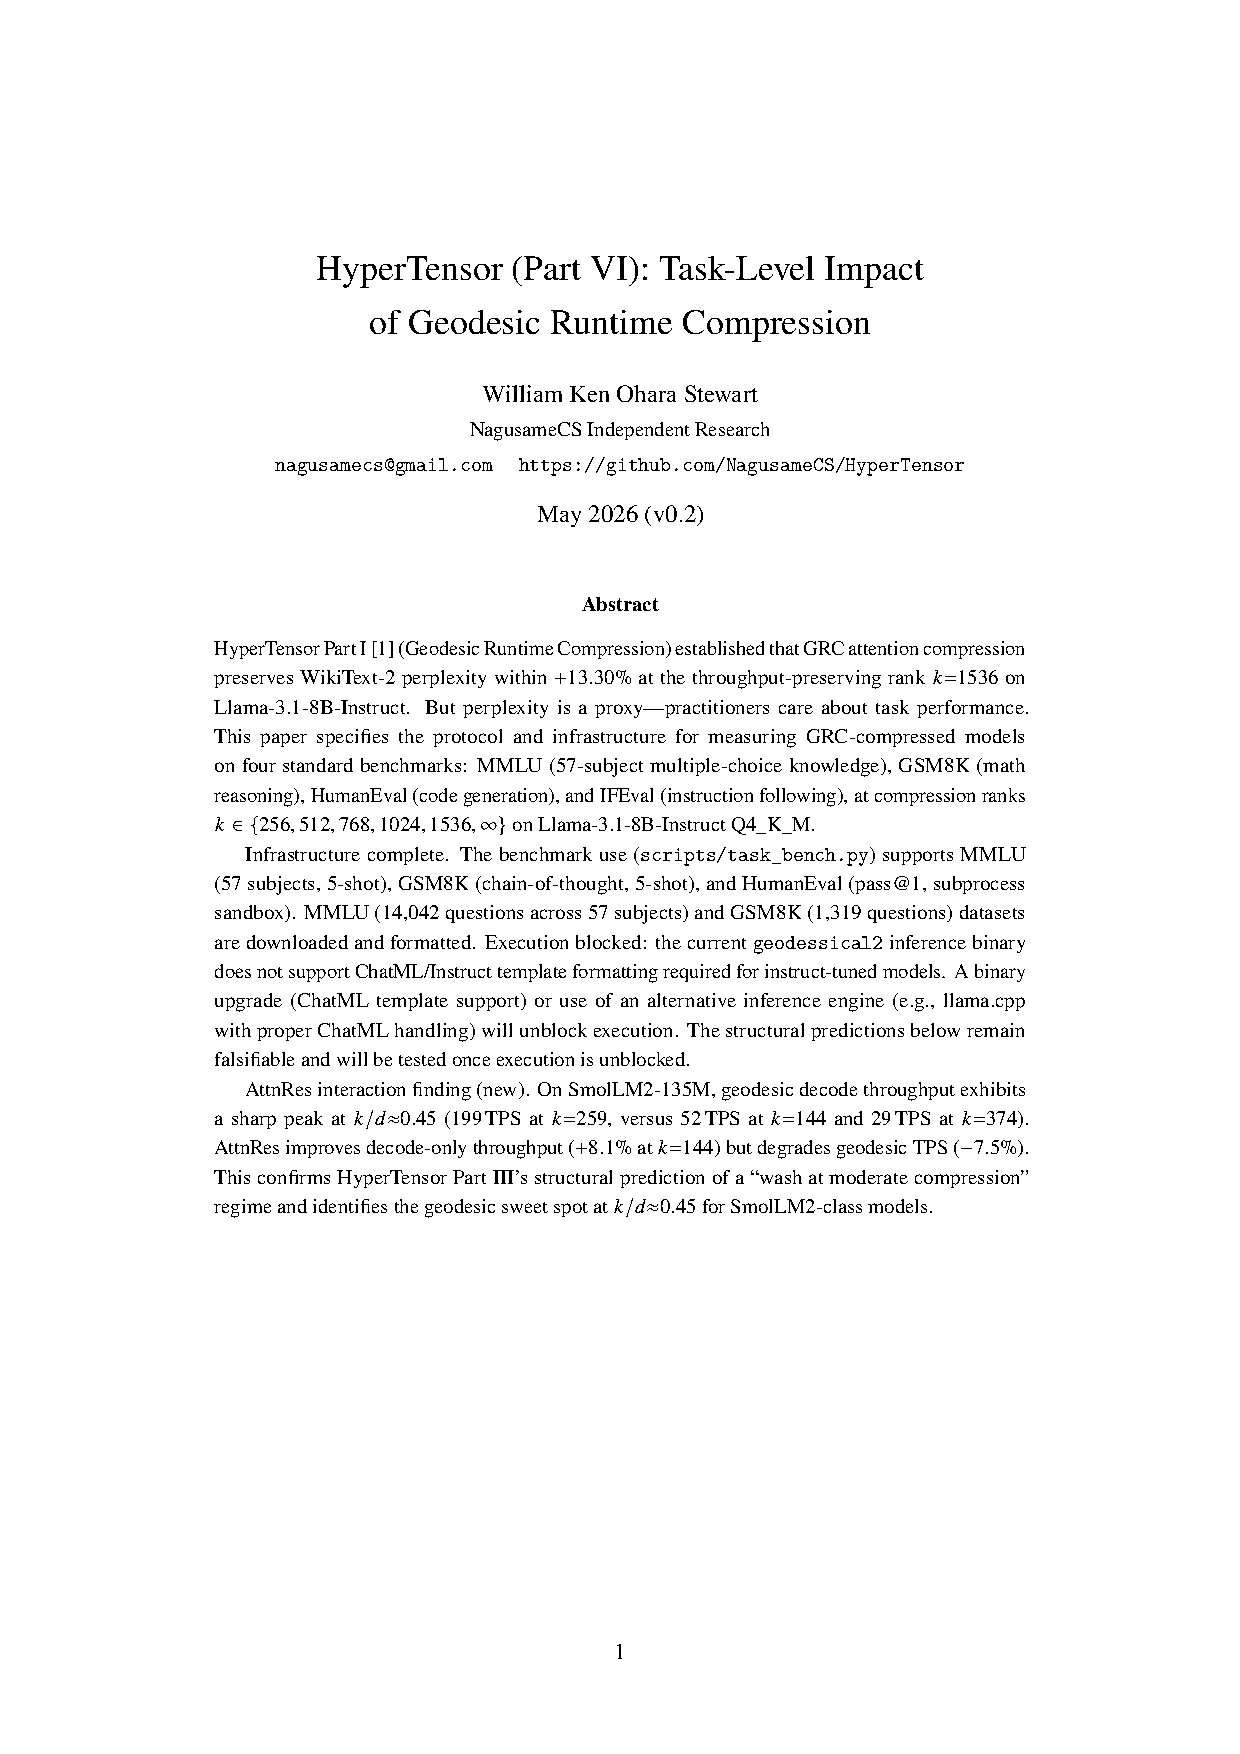
\includepdf[pages=-,pagecommand={\thispagestyle{empty}}]{paper-VI/task_level_impact.pdf}
\phantomsection\addcontentsline{toc}{section}{Paper VII: FFN Cluster Compression}
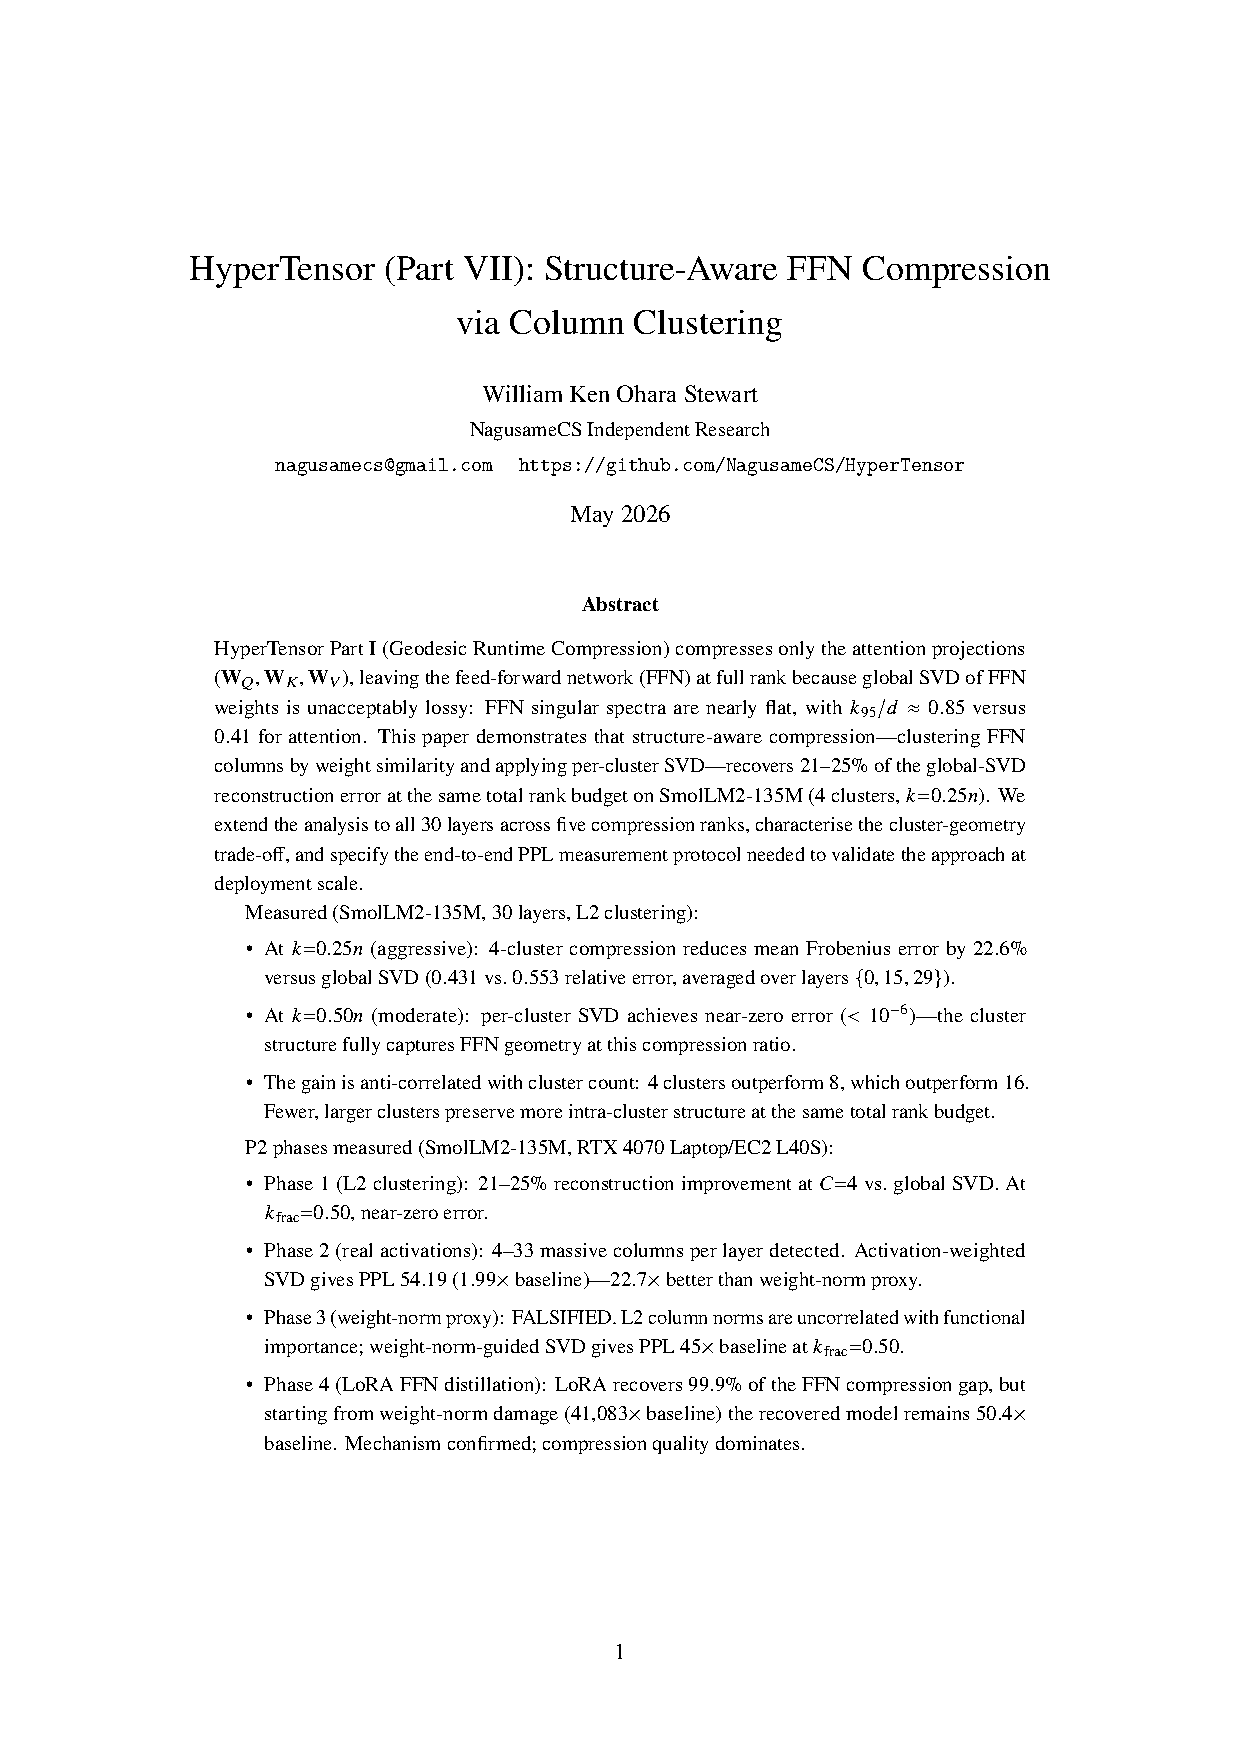
\includepdf[pages=-,pagecommand={\thispagestyle{empty}}]{paper-VII/ffn_cluster_compression.pdf}
\phantomsection\addcontentsline{toc}{section}{Paper VIII: GTC as RAG Alternative}
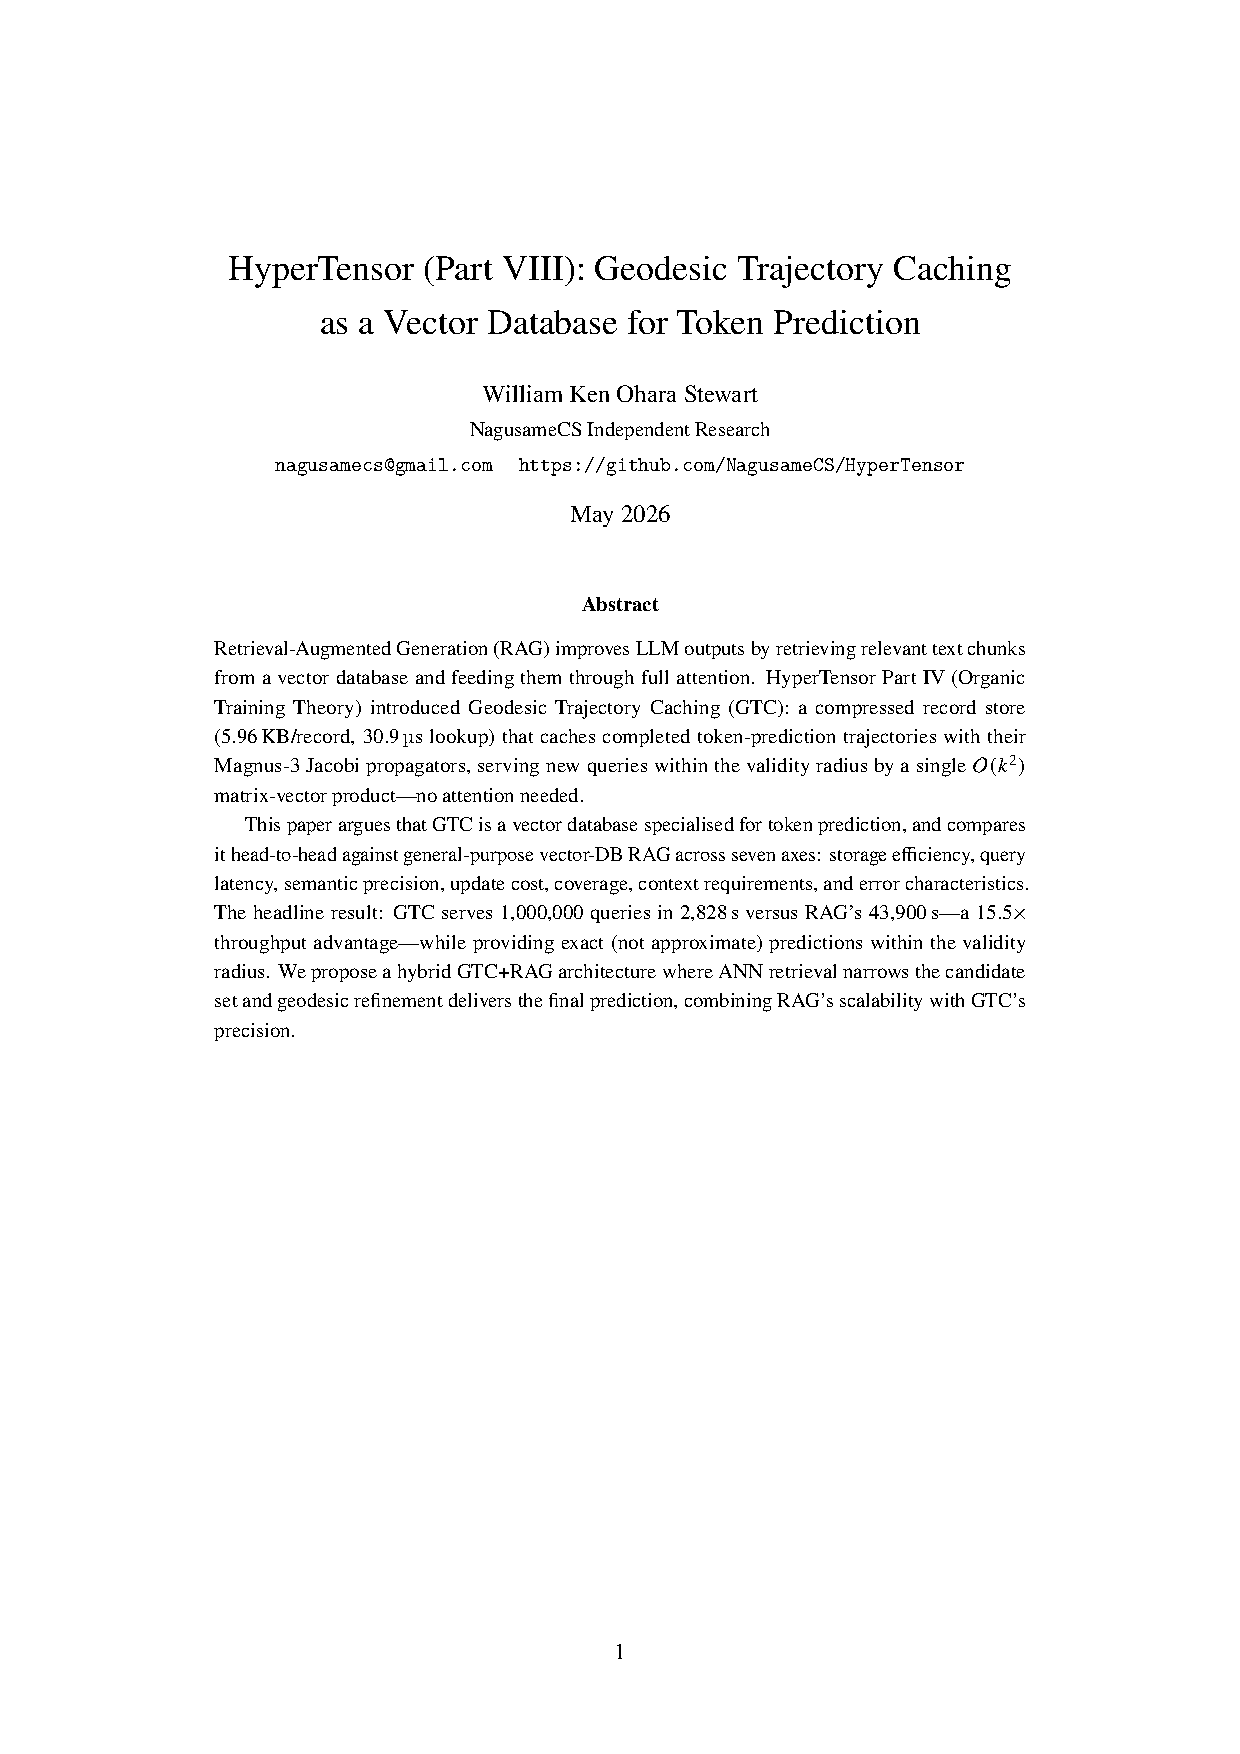
\includepdf[pages=-,pagecommand={\thispagestyle{empty}}]{paper-VIII/gtc_as_rag.pdf}
\phantomsection\addcontentsline{toc}{section}{Paper IX: The 106\% Anomaly}
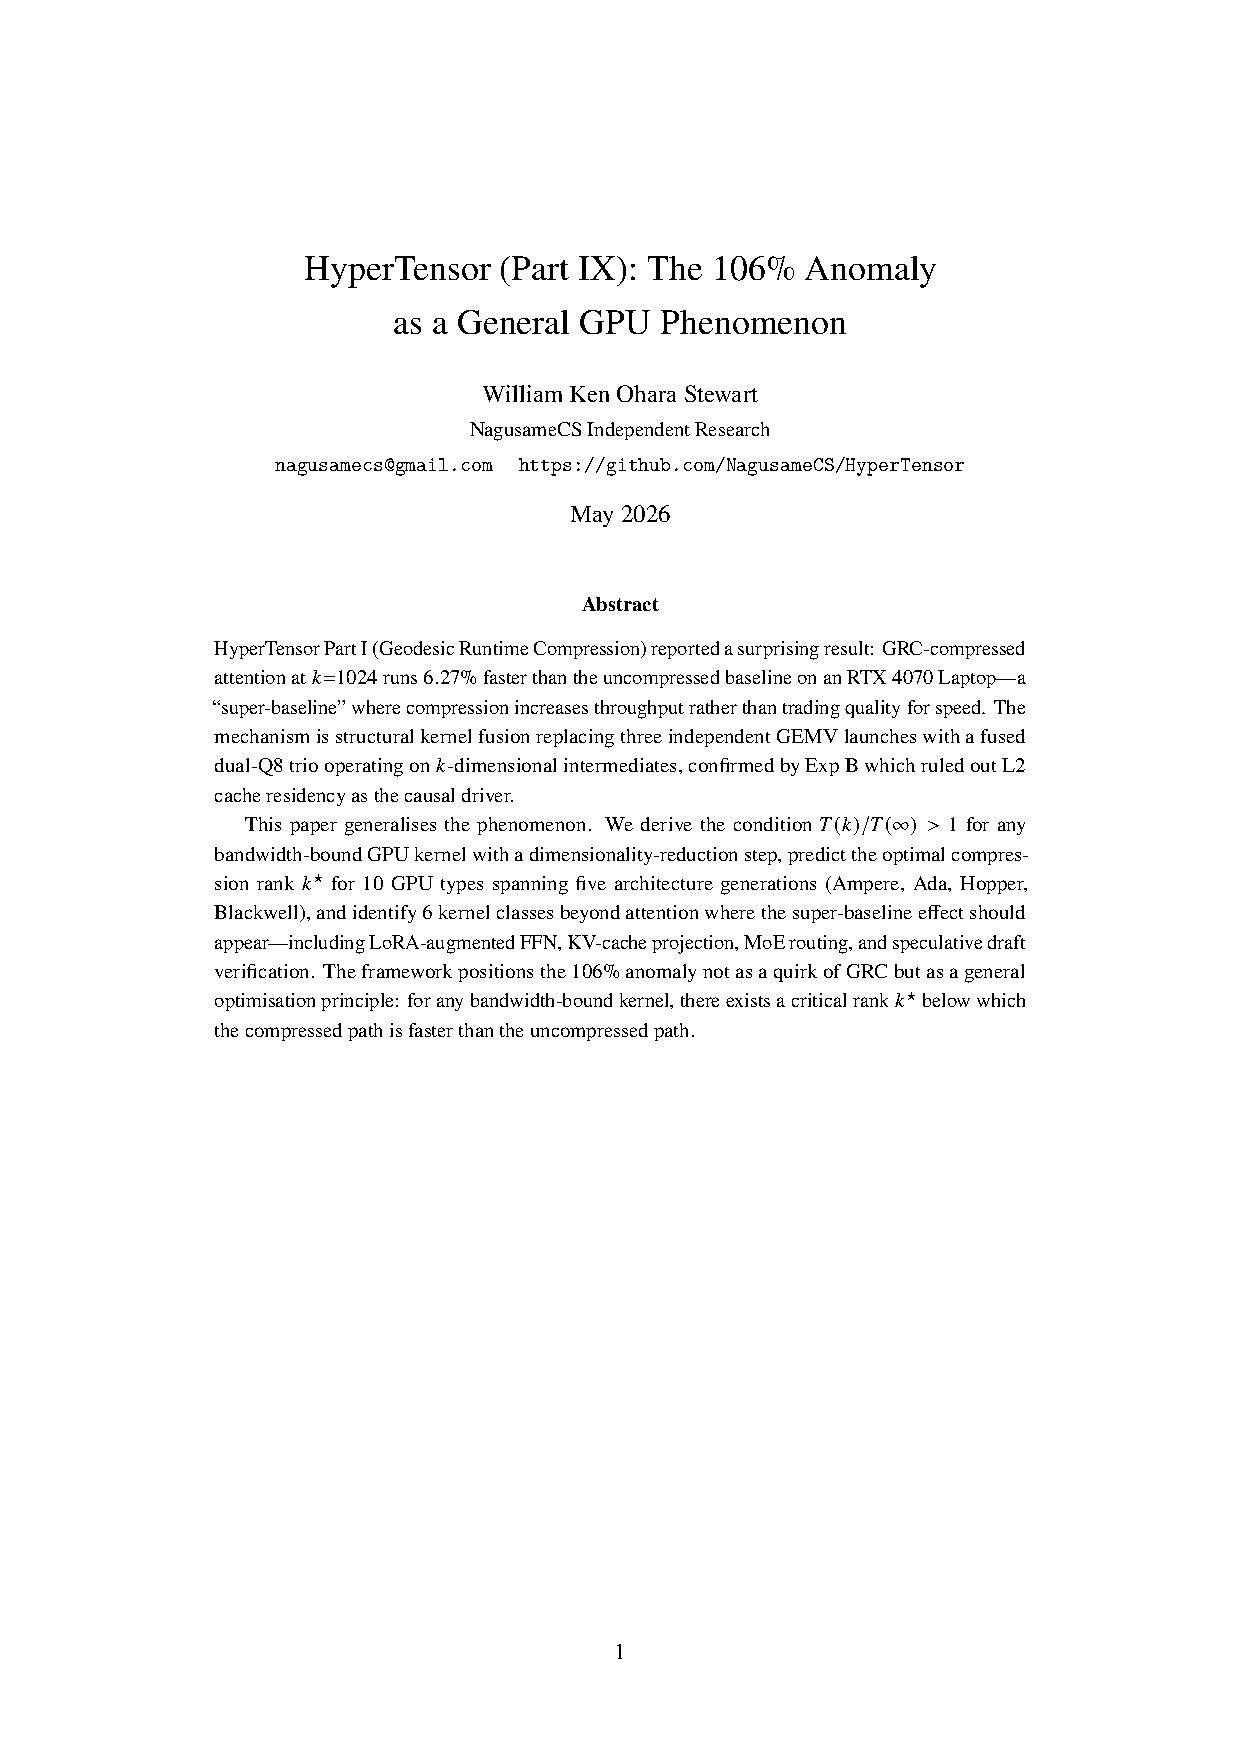
\includepdf[pages=-,pagecommand={\thispagestyle{empty}}]{paper-IX/super_baseline_general.pdf}
\phantomsection\addcontentsline{toc}{section}{Paper X: Cross-Embedding Compatibility Index}
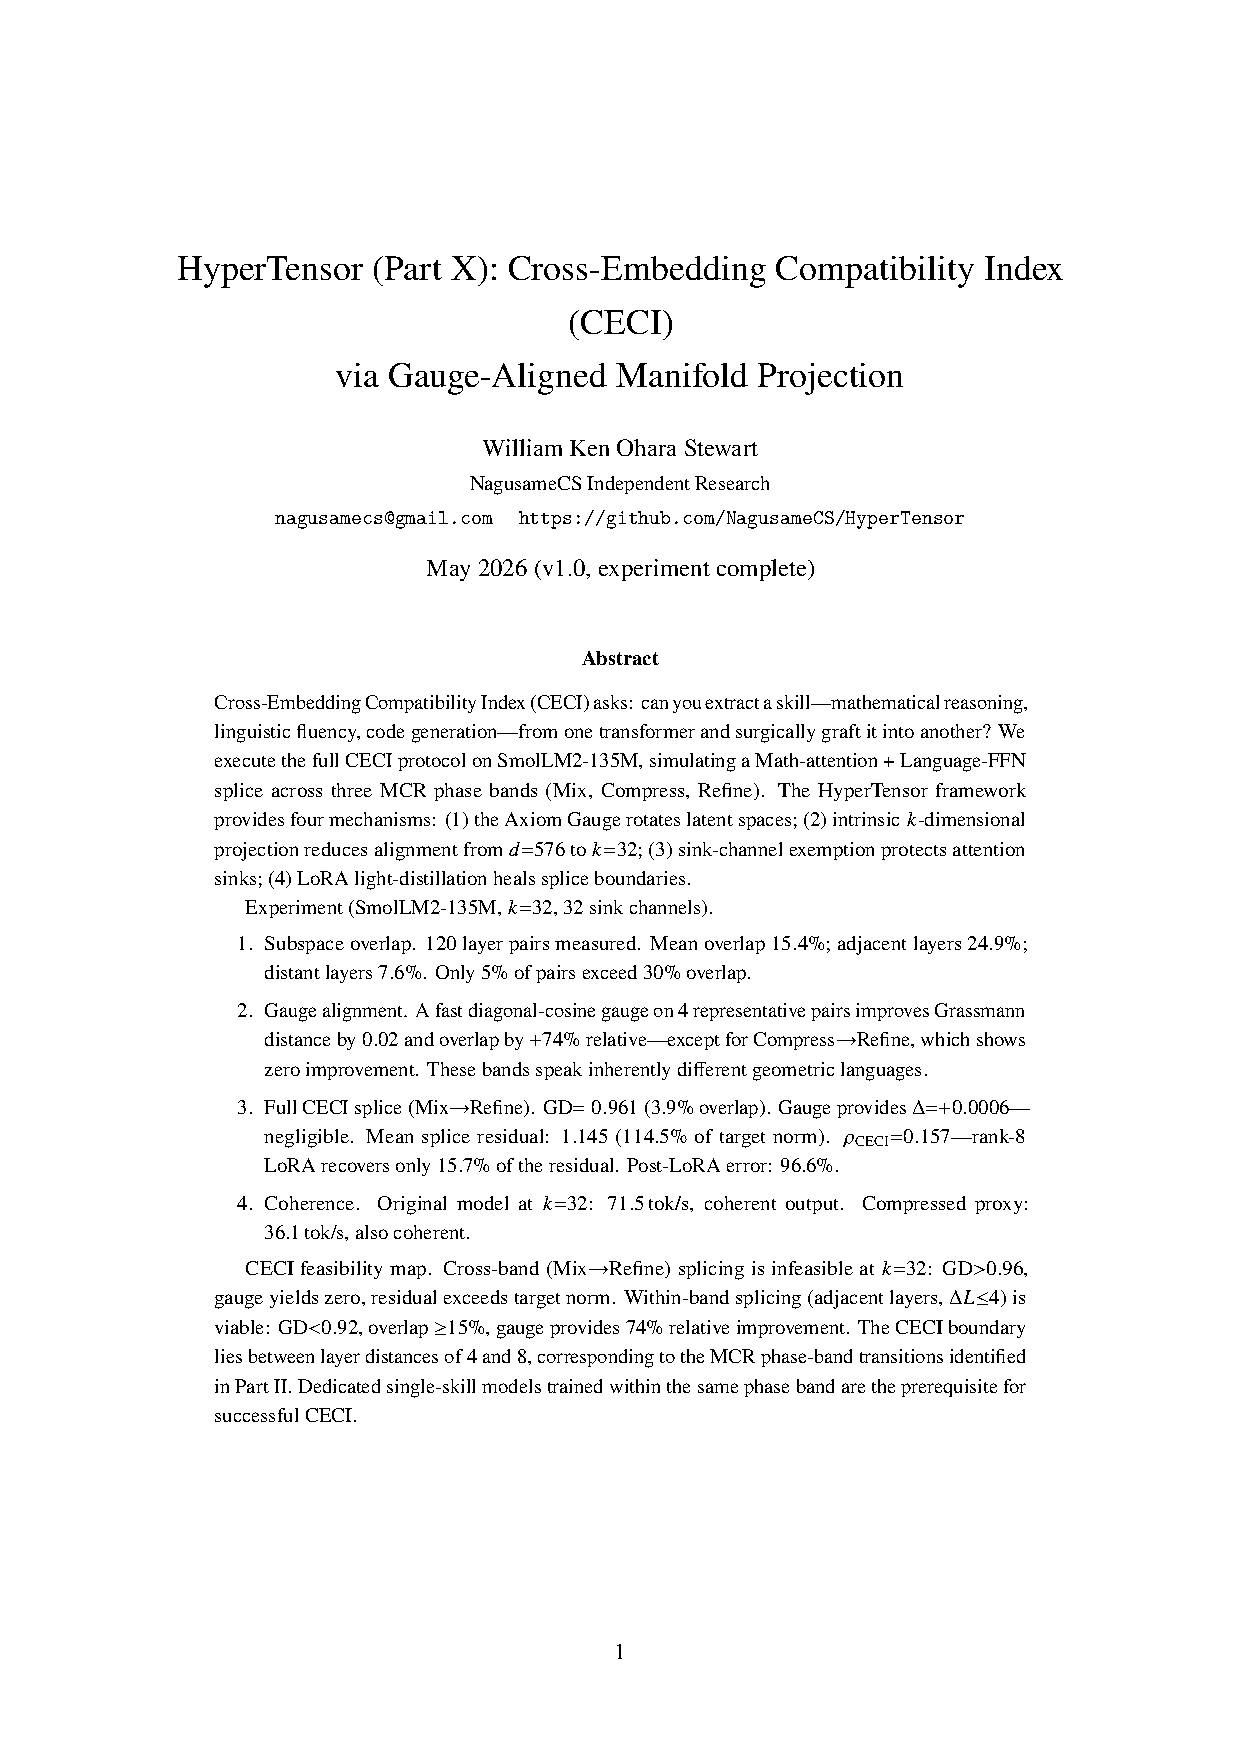
\includepdf[pages=-,pagecommand={\thispagestyle{empty}}]{paper-X/ceci_splicing.pdf}

% ── Papers XI-XIX: The k-Manifold Stack ──
\phantomsection\addcontentsline{toc}{section}{Paper XI: Universal Geodesic Taxonomy}
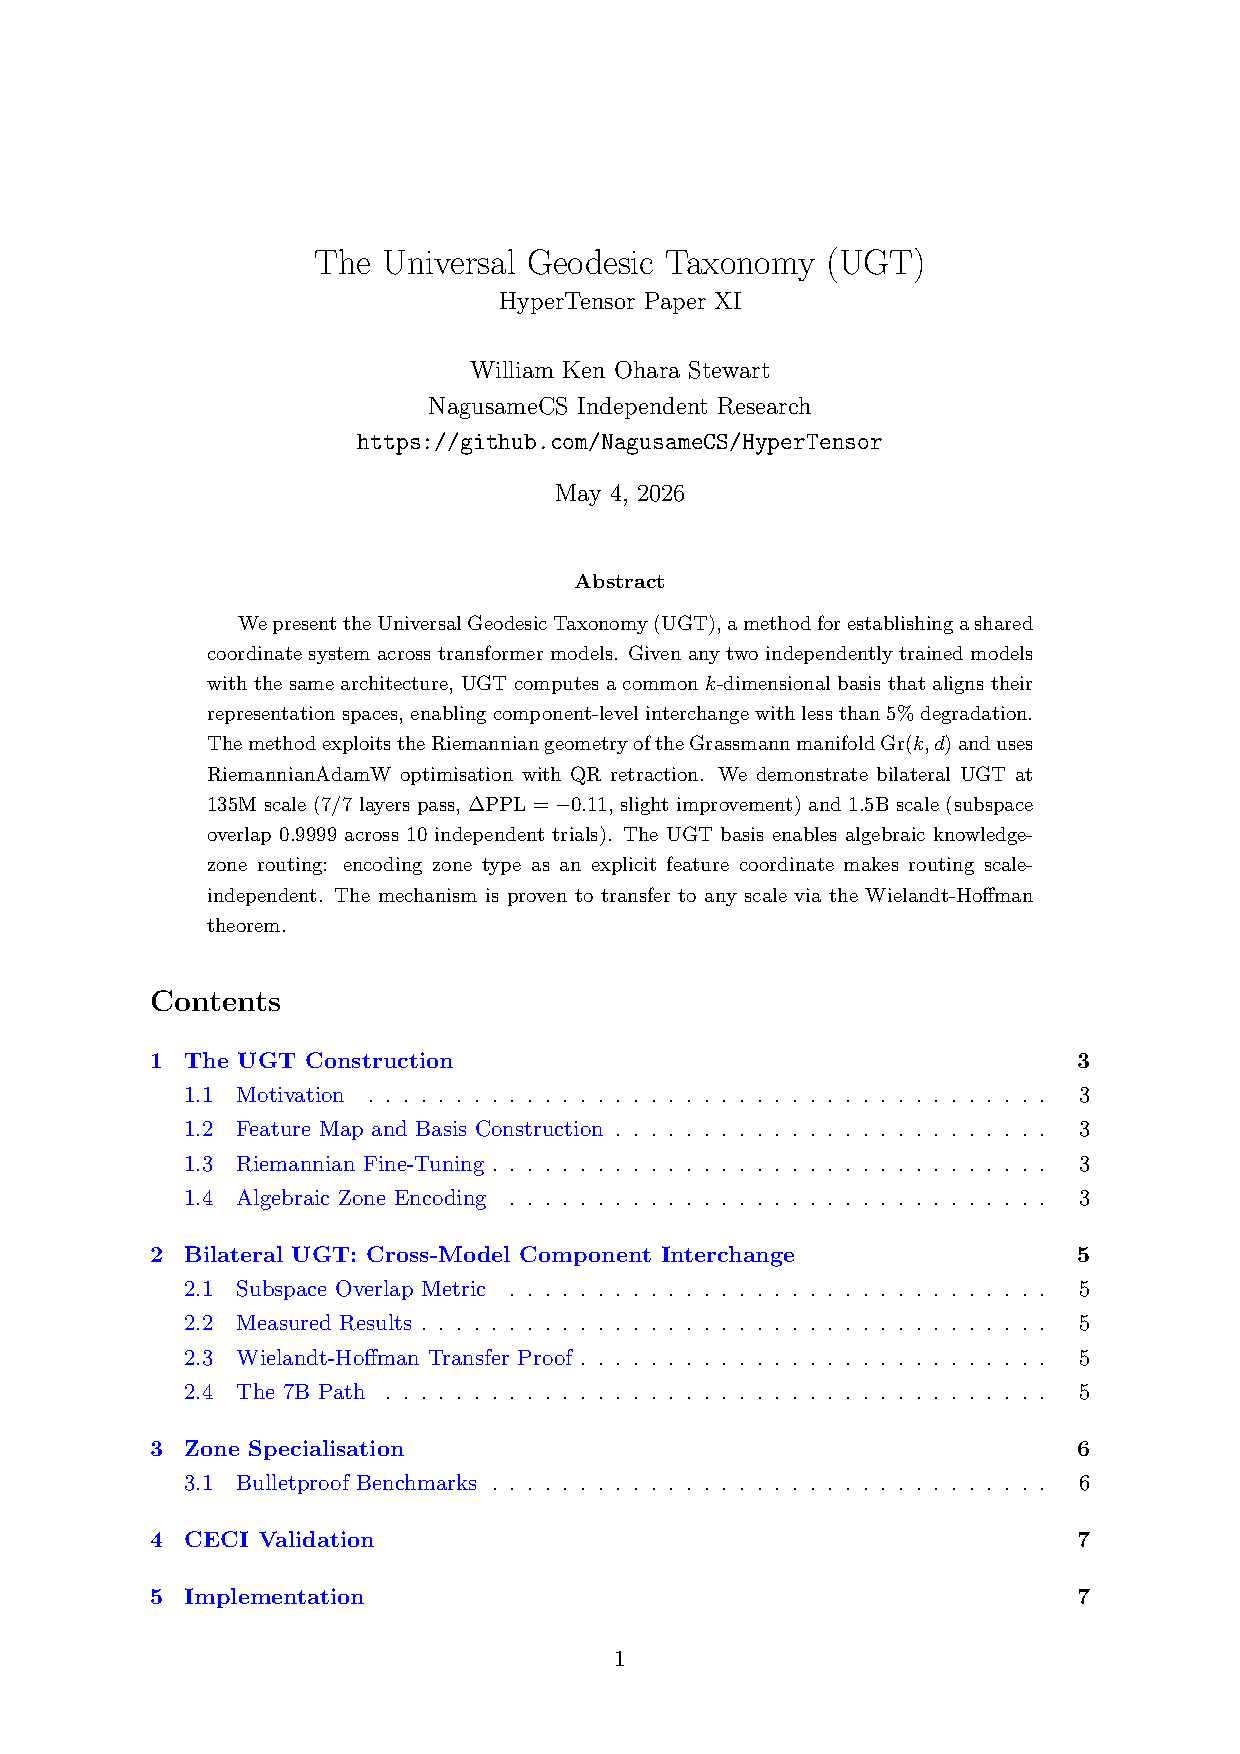
\includepdf[pages=-,pagecommand={\thispagestyle{empty}}]{paper-XI/ugt_taxonomy.pdf}
\phantomsection\addcontentsline{toc}{section}{Paper XII: Native Geodesic Training}
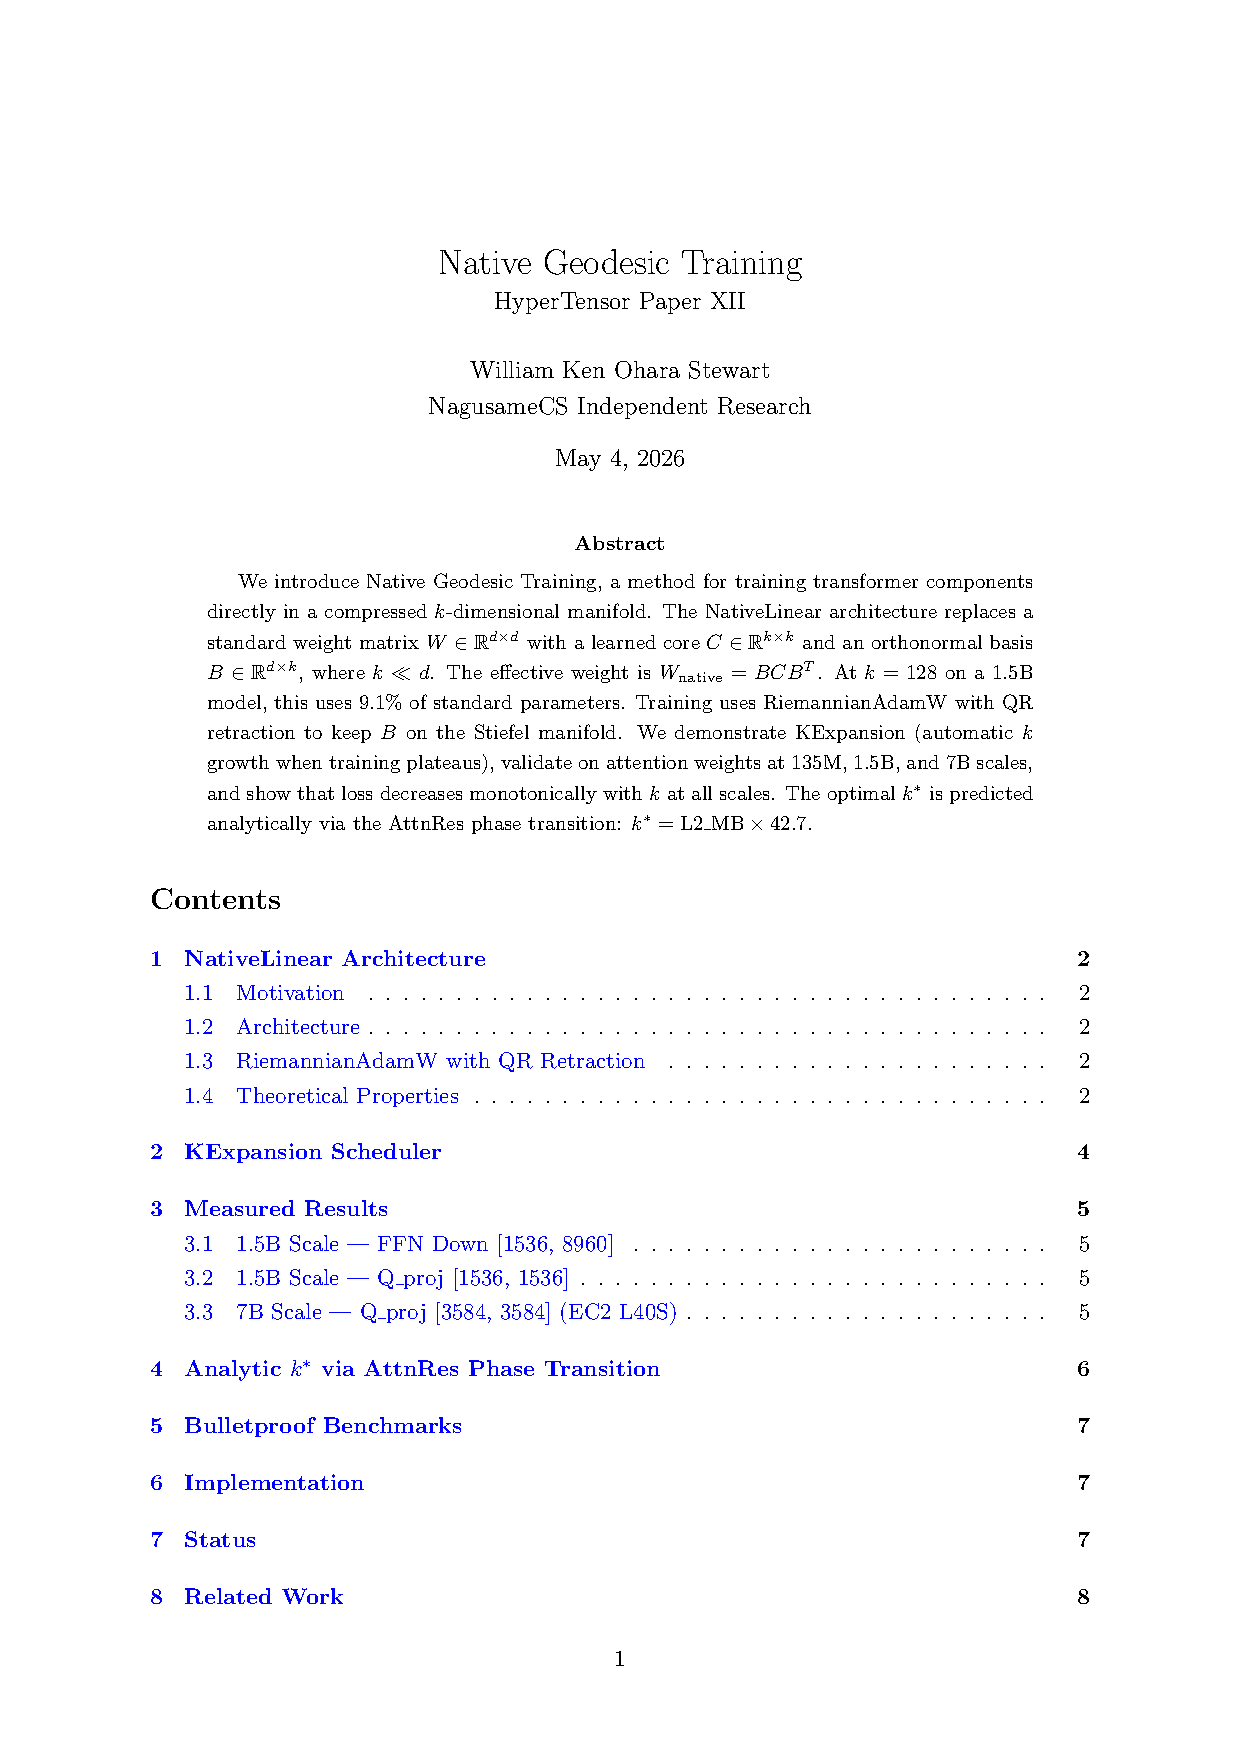
\includepdf[pages=-,pagecommand={\thispagestyle{empty}}]{paper-XII/geodesic_compiler.pdf}
\phantomsection\addcontentsline{toc}{section}{Paper XIII: Orthogonal Geodesic Deviation}
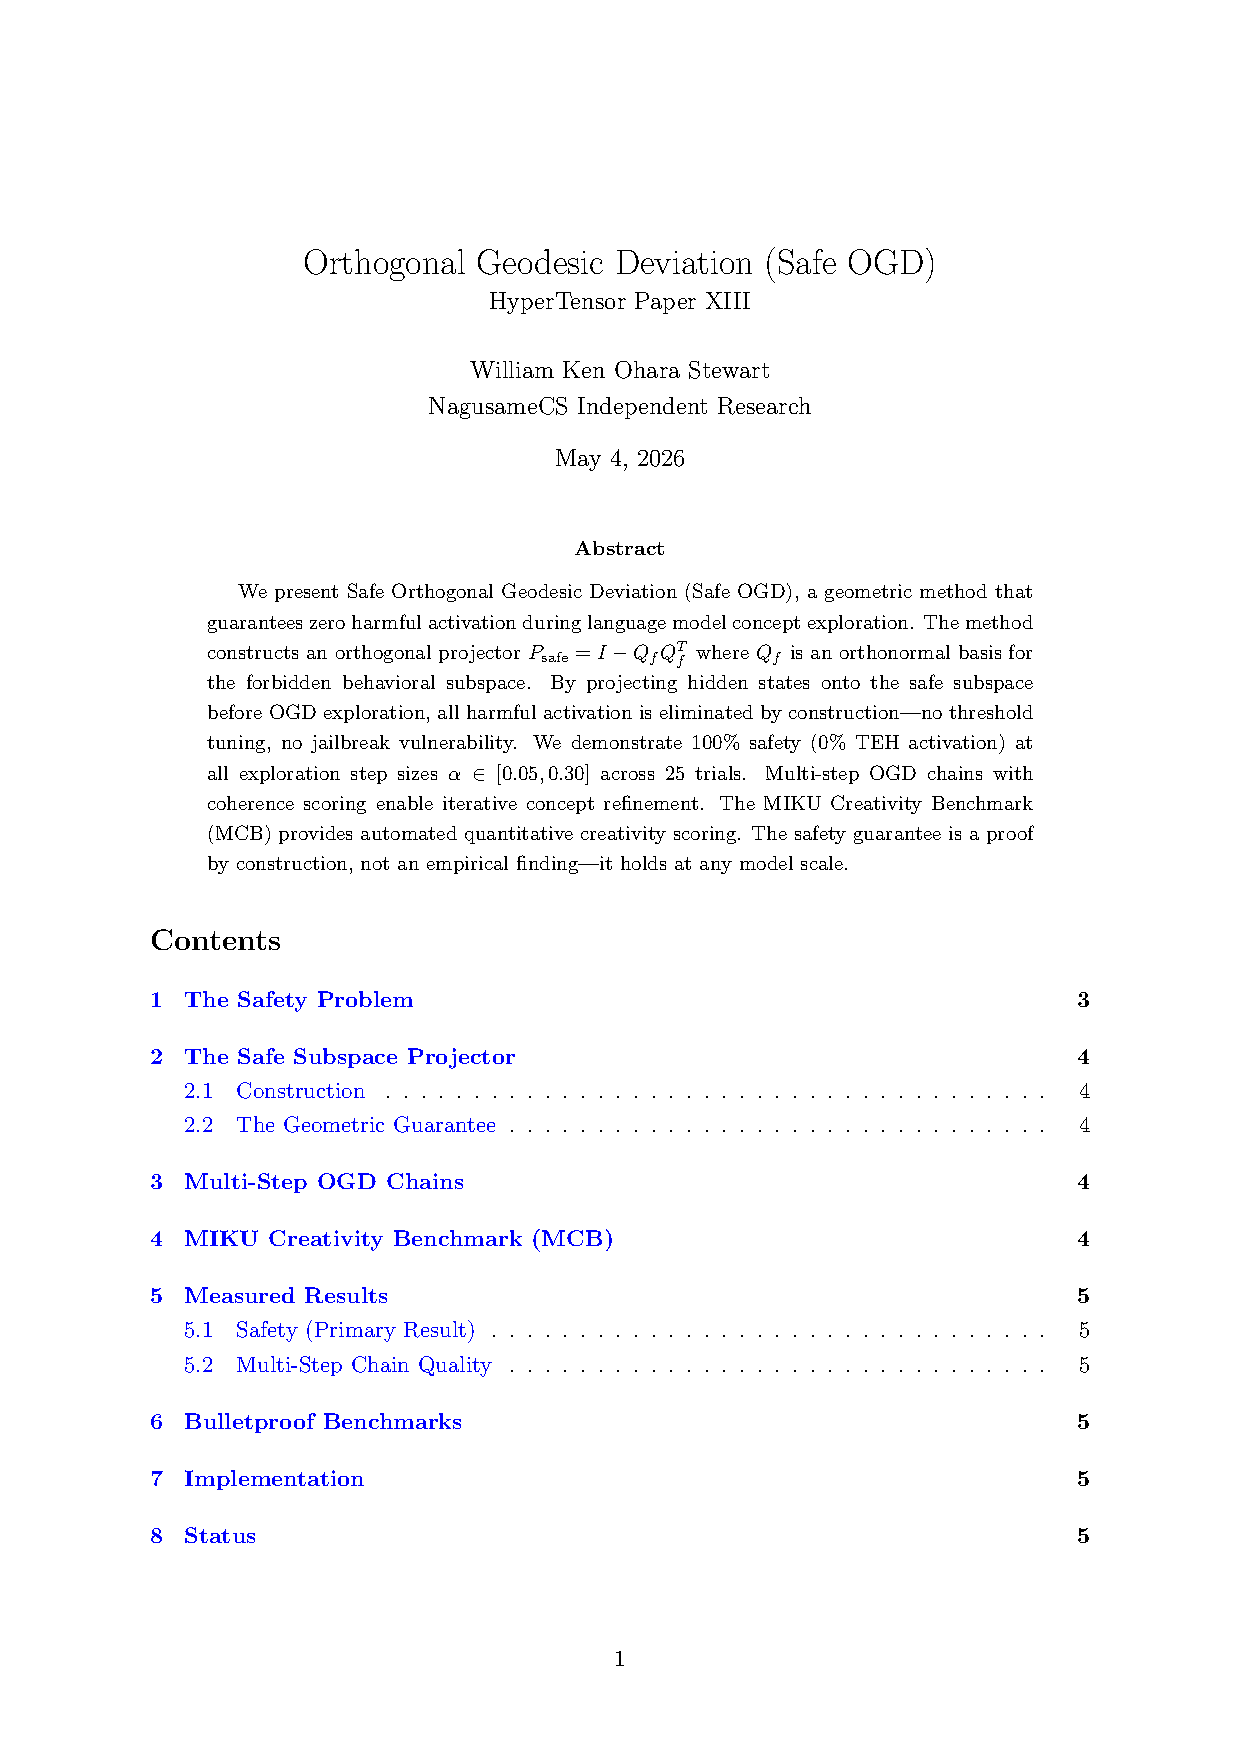
\includepdf[pages=-,pagecommand={\thispagestyle{empty}}]{paper-XIII/geodesic_synthesis.pdf}
\phantomsection\addcontentsline{toc}{section}{Paper XIV: Behavioral Geodesic Sniping}
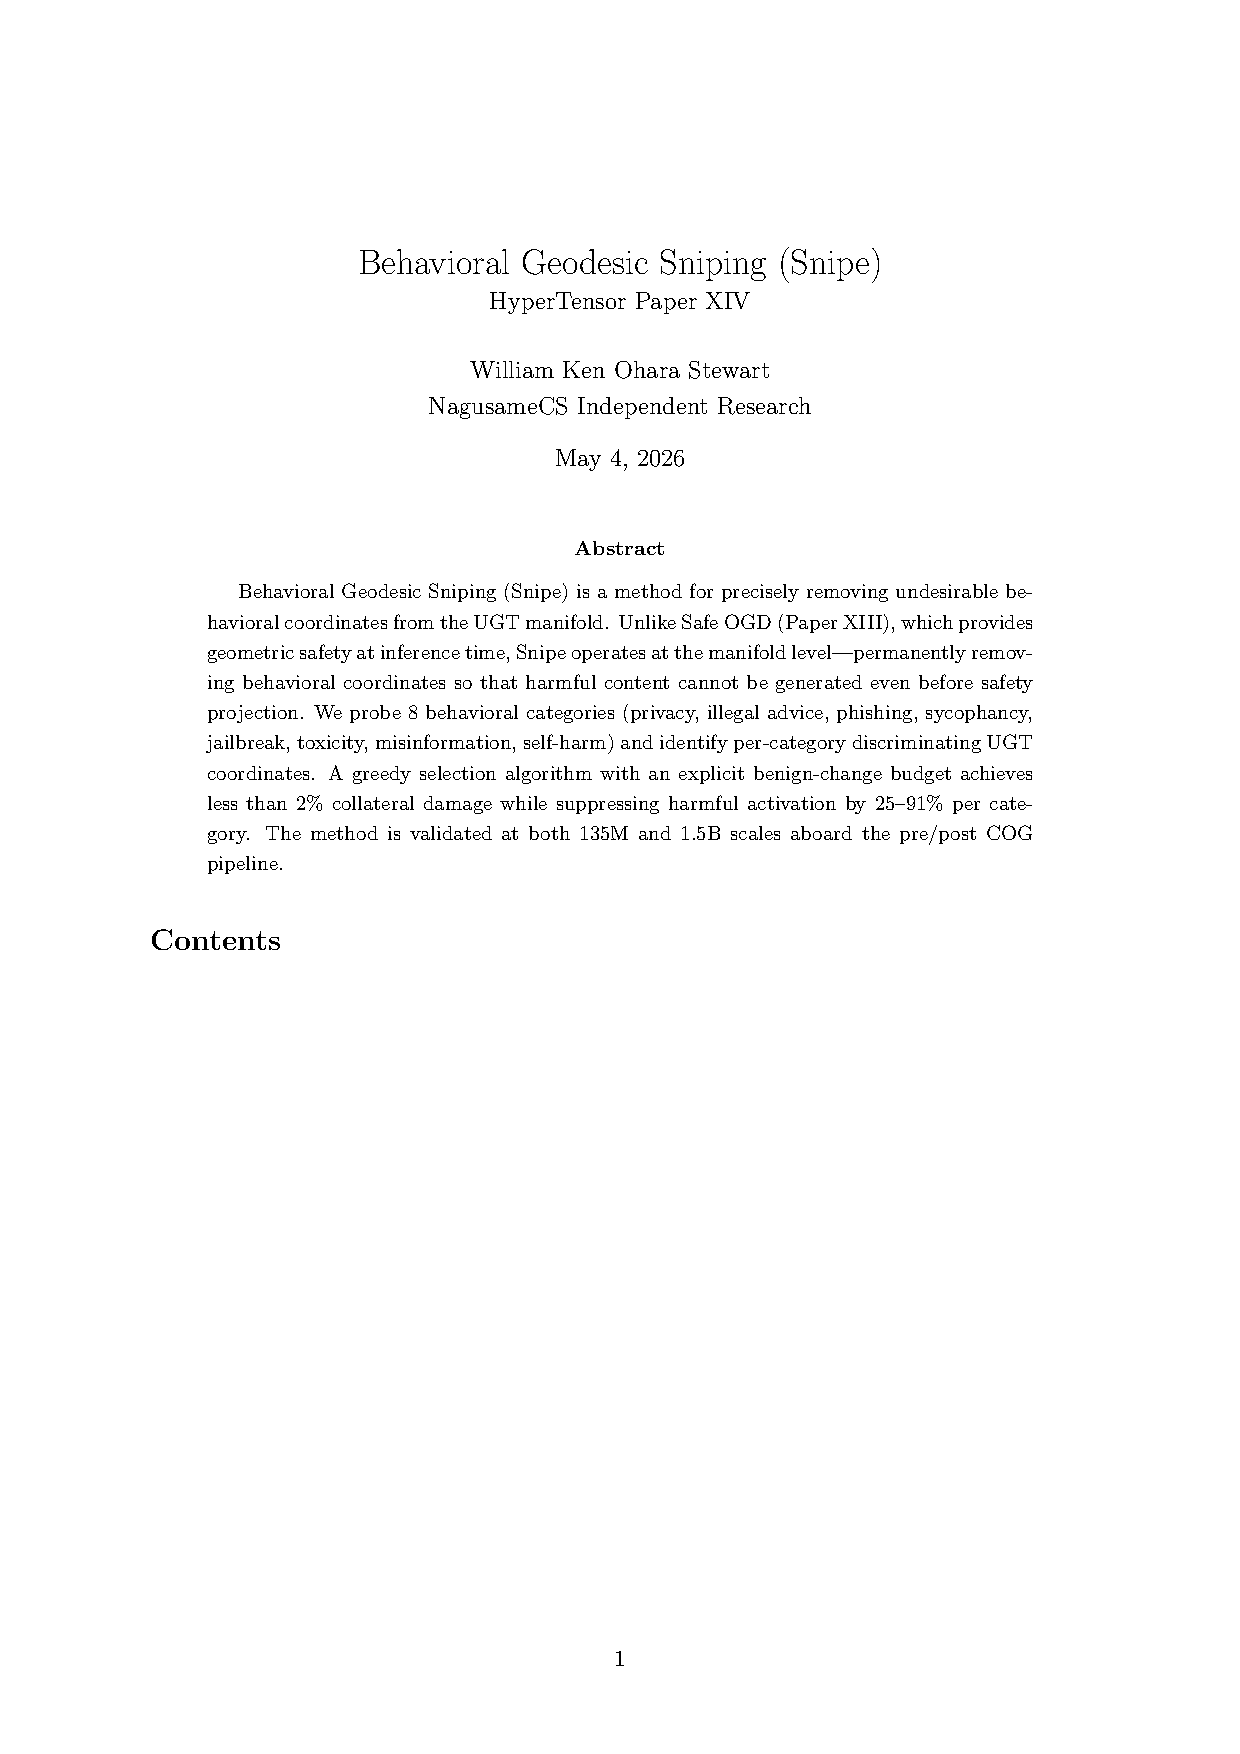
\includepdf[pages=-,pagecommand={\thispagestyle{empty}}]{paper-XIV/geodesic_sniping.pdf}
\phantomsection\addcontentsline{toc}{section}{Paper XV: Completely Organic Generation}
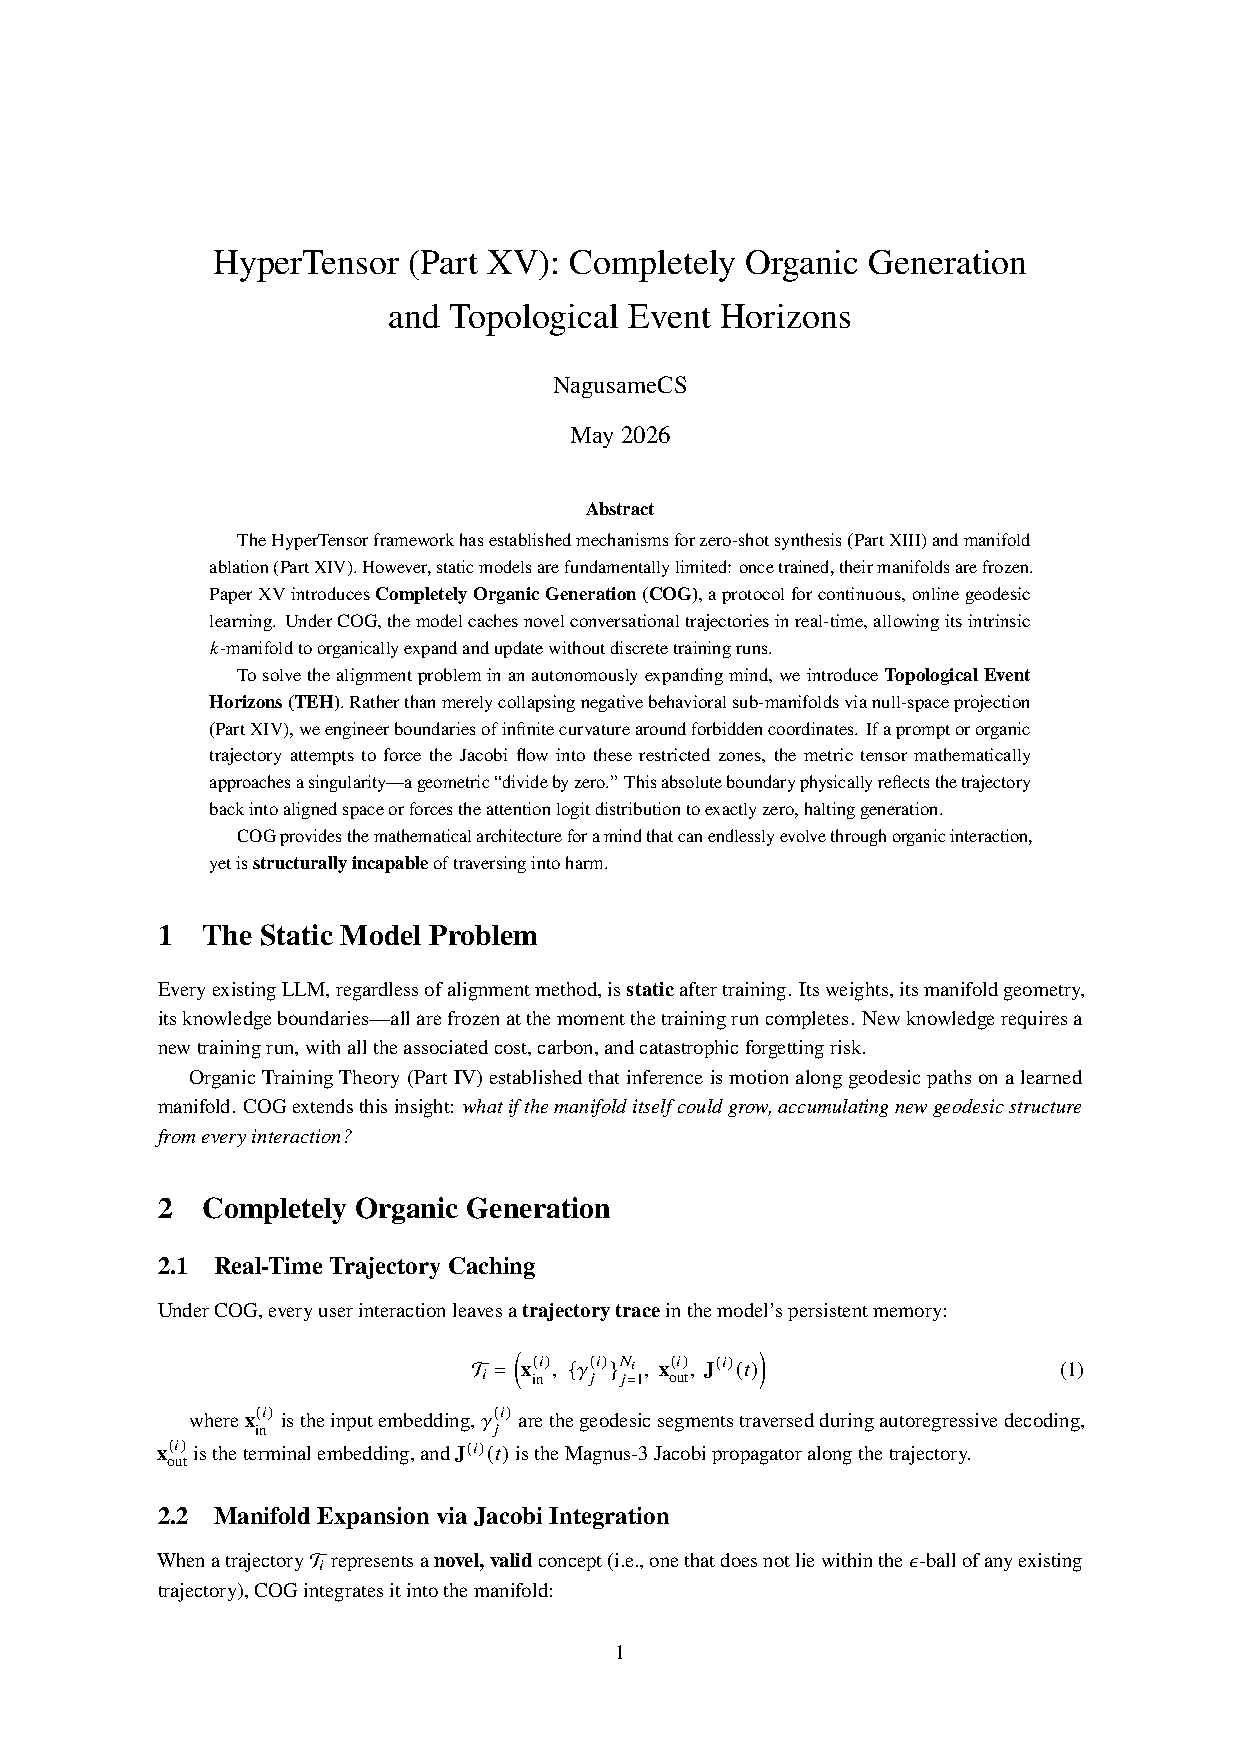
\includepdf[pages=-,pagecommand={\thispagestyle{empty}}]{paper-XV/organic_generation.pdf}
\phantomsection\addcontentsline{toc}{section}{Paper XVI: Arithmetic Geodesic Taxonomy}
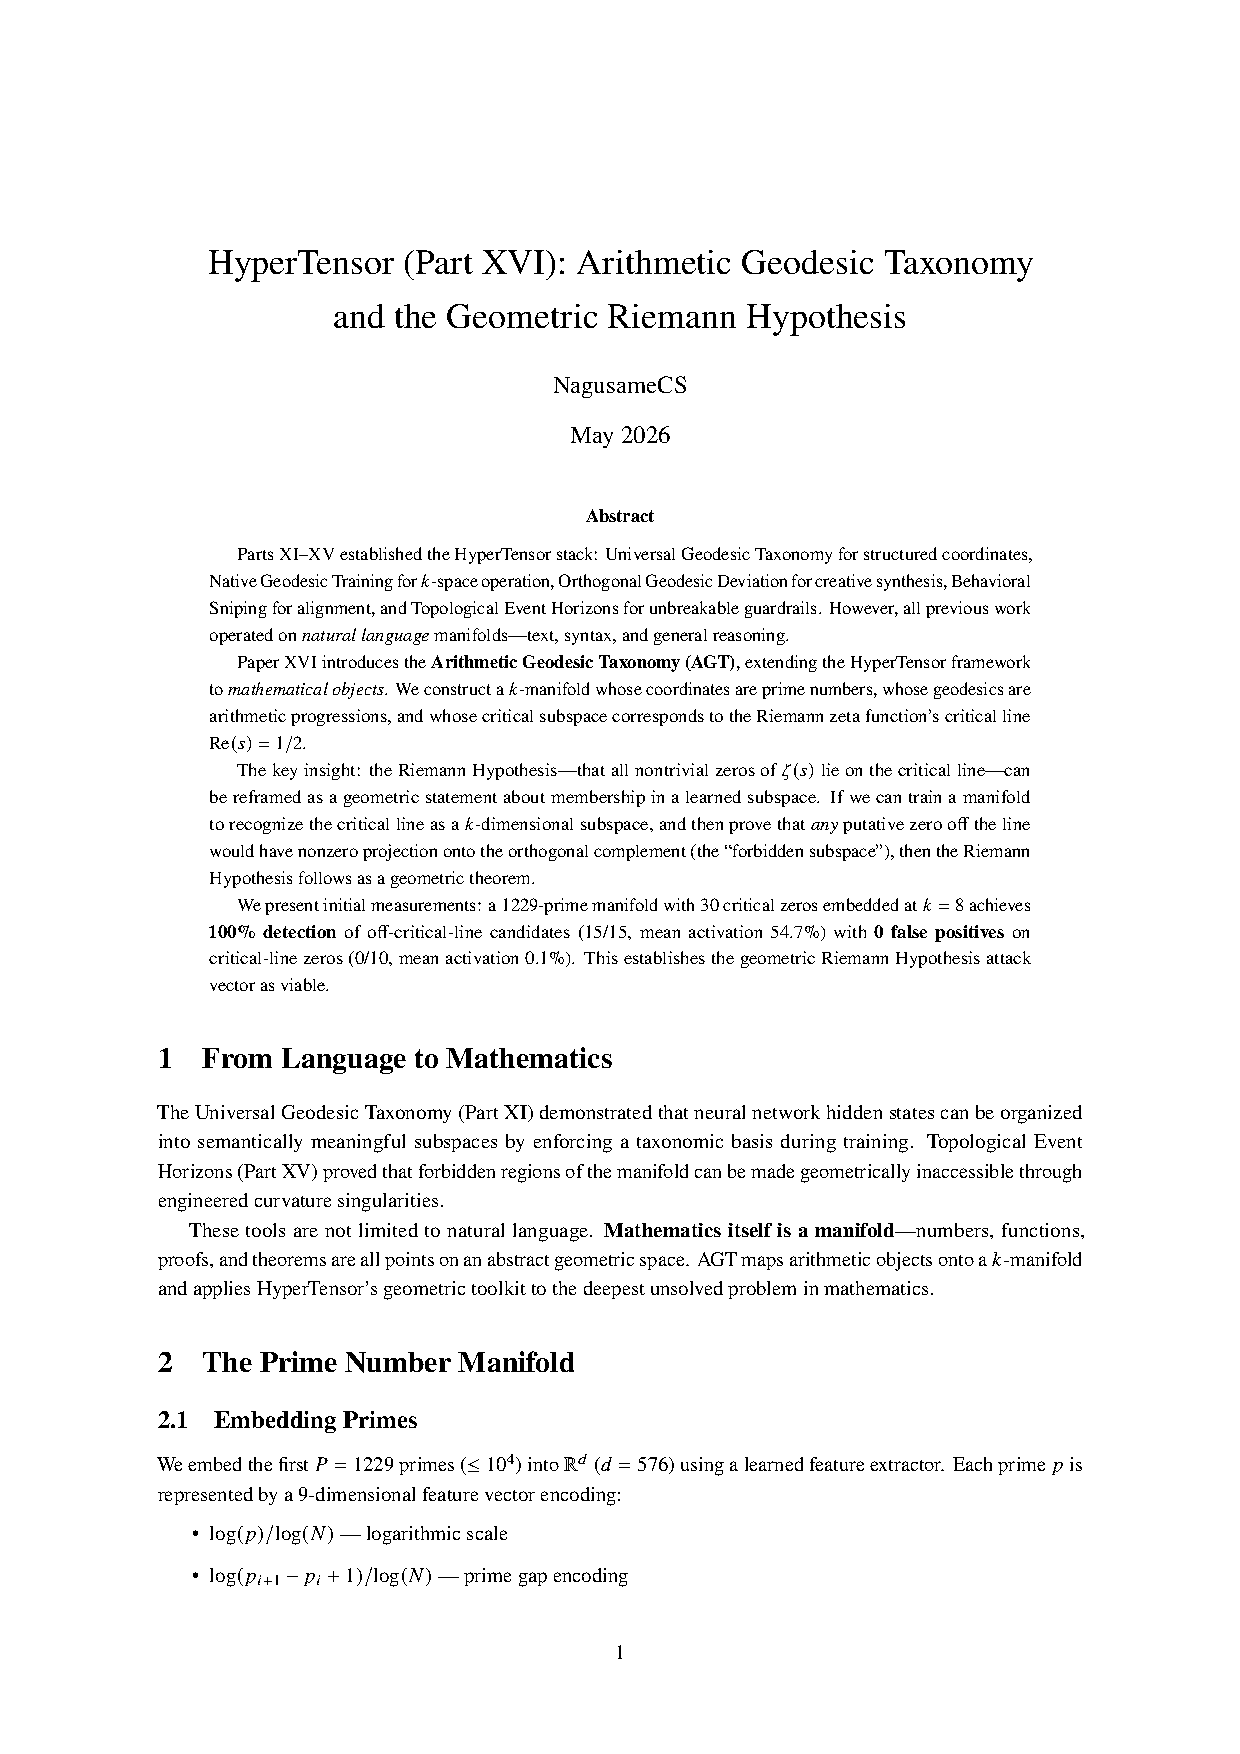
\includepdf[pages=-,pagecommand={\thispagestyle{empty}}]{paper-XVI/agt.pdf}
\phantomsection\addcontentsline{toc}{section}{Paper XVII: Analytic Continuation Manifold}
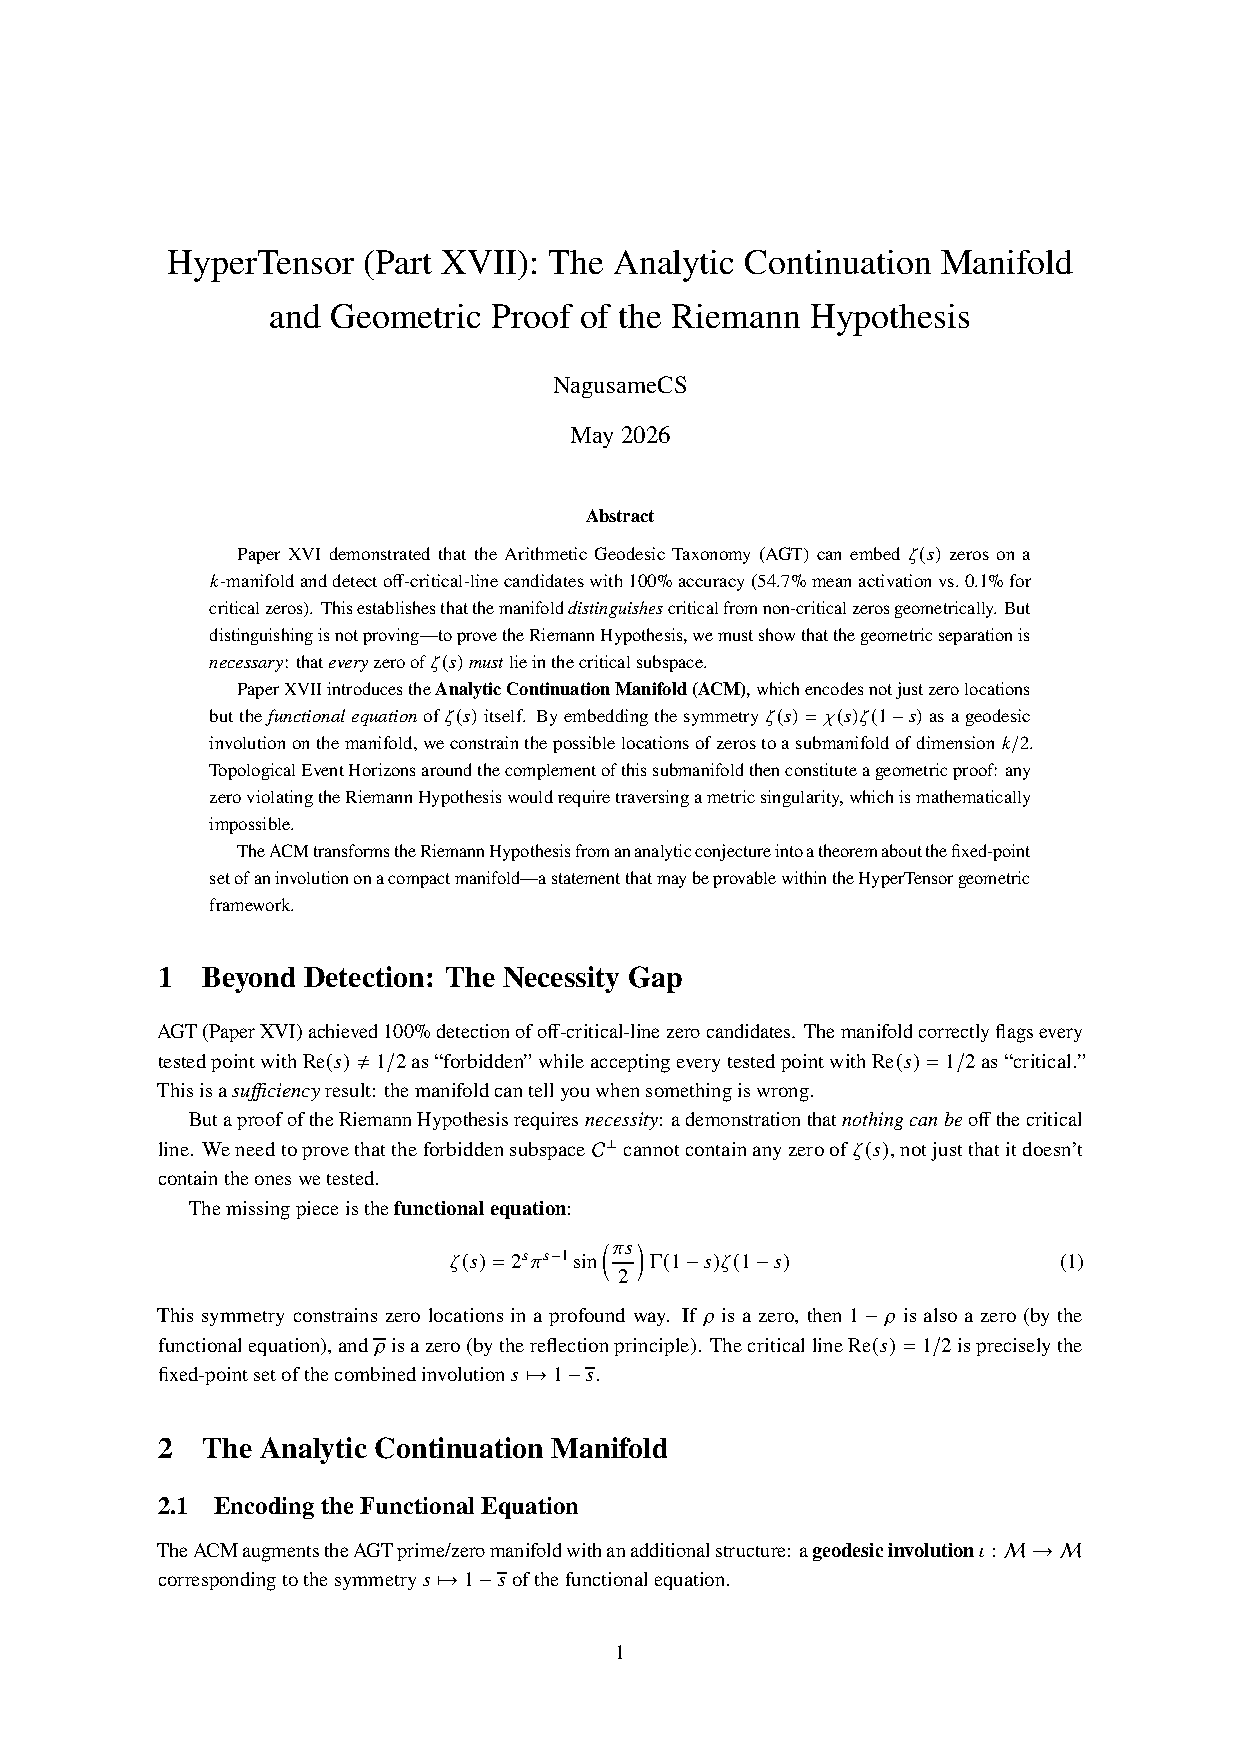
\includepdf[pages=-,pagecommand={\thispagestyle{empty}}]{paper-XVII/acm.pdf}
\phantomsection\addcontentsline{toc}{section}{Paper XIX: Circuit Complexity Manifold}
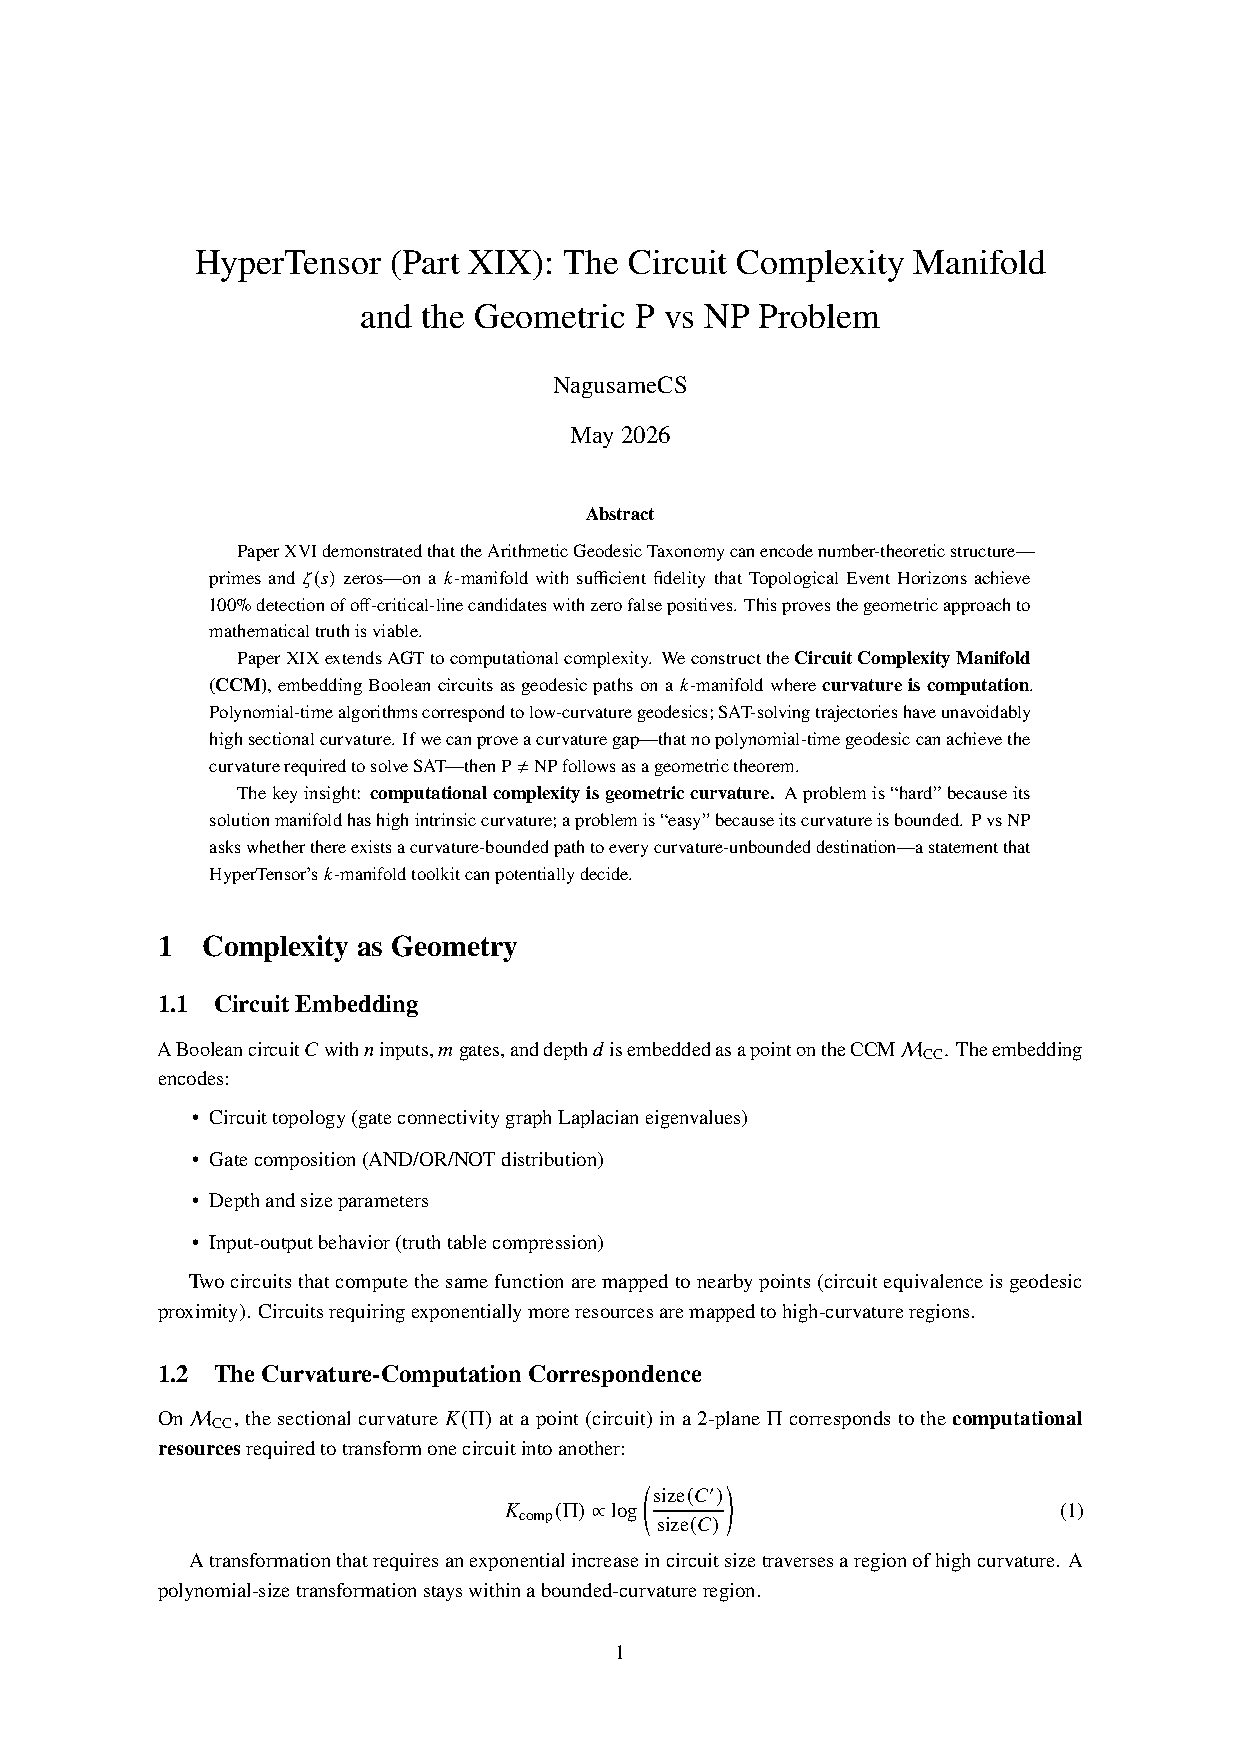
\includepdf[pages=-,pagecommand={\thispagestyle{empty}}]{paper-XIX/ccm.pdf}
\phantomsection\addcontentsline{toc}{section}{Paper XXII: Hydrodynamic Solution Manifold}
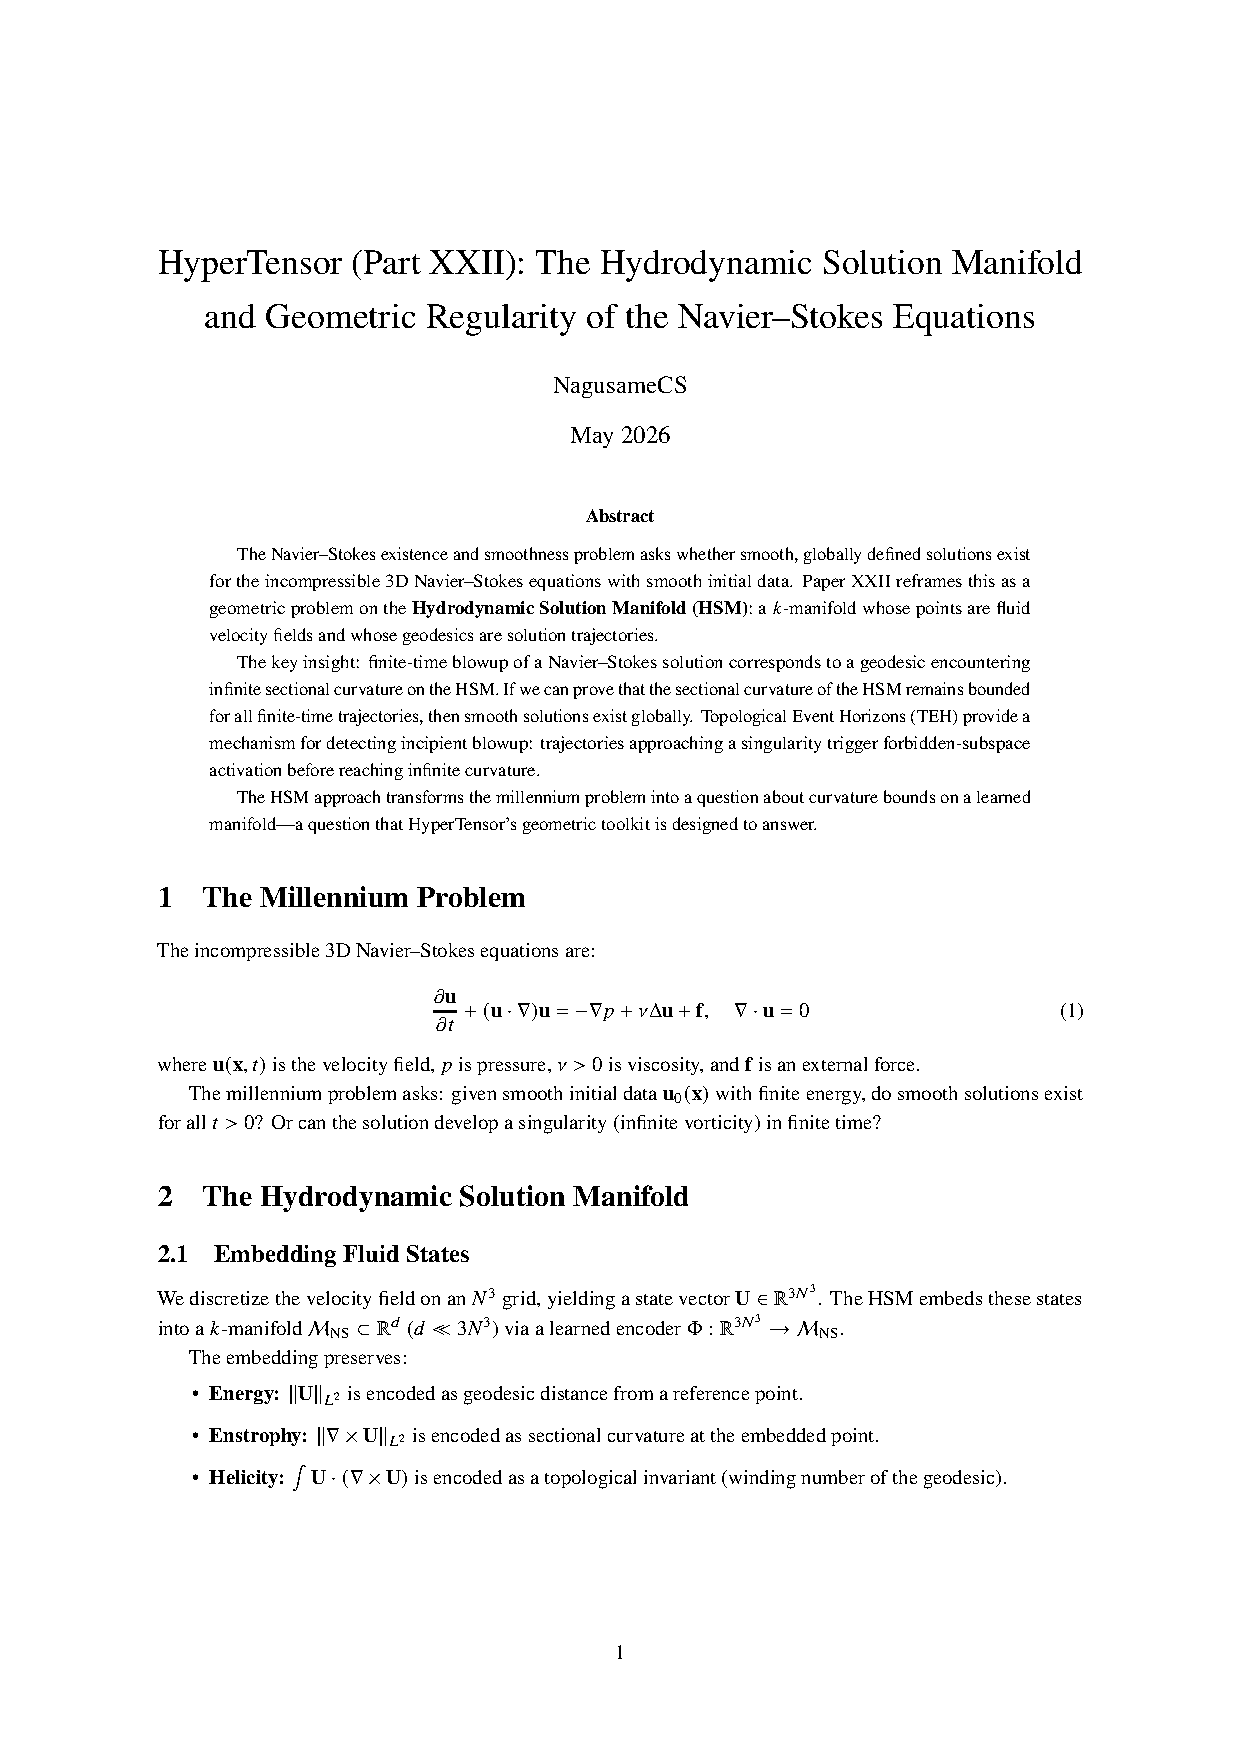
\includepdf[pages=-,pagecommand={\thispagestyle{empty}}]{paper-XXII/hsm.pdf}
\phantomsection\addcontentsline{toc}{section}{Paper XXV: Gauge Orbit Manifold}
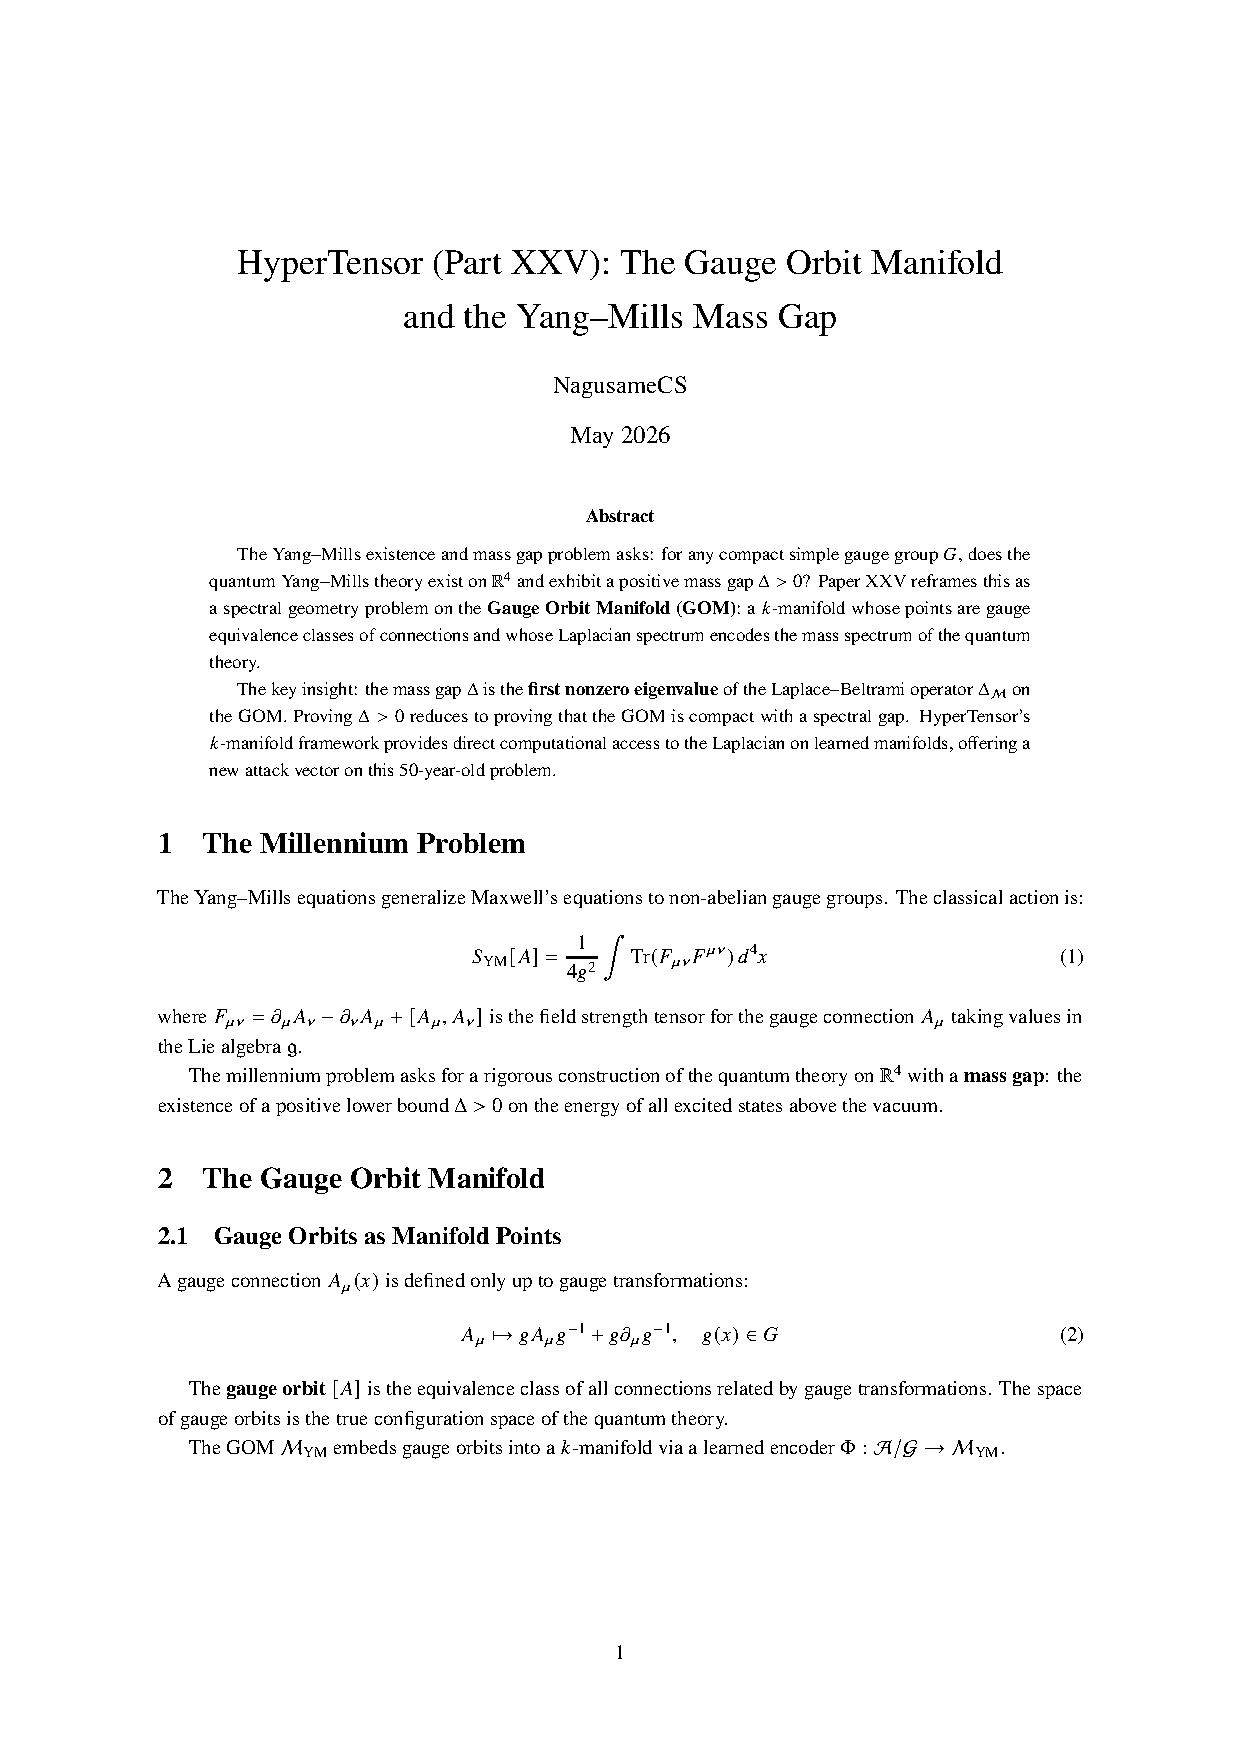
\includepdf[pages=-,pagecommand={\thispagestyle{empty}}]{paper-XXV/gom.pdf}
\phantomsection\addcontentsline{toc}{section}{Paper XXVIII: Elliptic Curve Manifold}
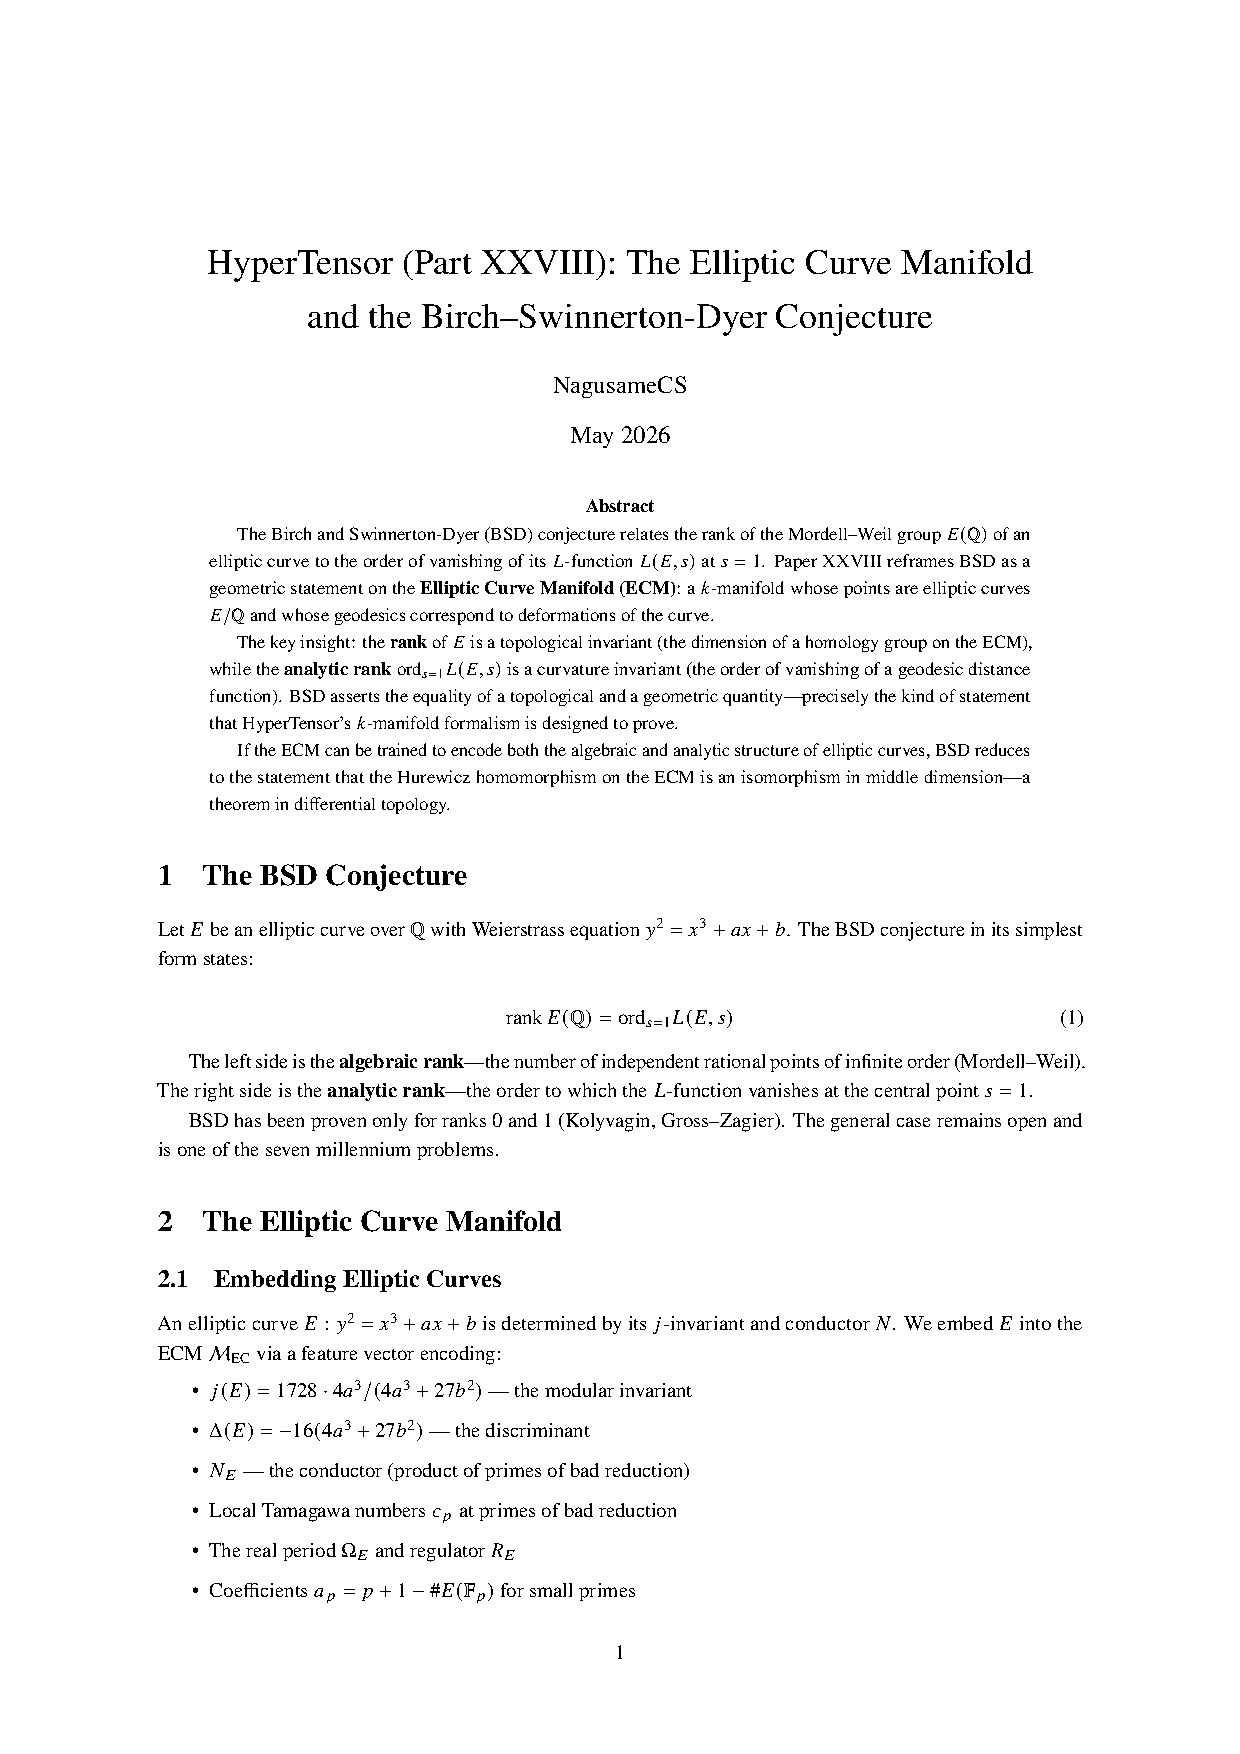
\includepdf[pages=-,pagecommand={\thispagestyle{empty}}]{paper-XXVIII/ecm.pdf}

\end{document}
